% Options for packages loaded elsewhere
\PassOptionsToPackage{unicode}{hyperref}
\PassOptionsToPackage{hyphens}{url}
%
\documentclass[
  english,
  jou]{apa7}
\usepackage{lmodern}
\usepackage{amsmath}
\usepackage{ifxetex,ifluatex}
\ifnum 0\ifxetex 1\fi\ifluatex 1\fi=0 % if pdftex
  \usepackage[T1]{fontenc}
  \usepackage[utf8]{inputenc}
  \usepackage{textcomp} % provide euro and other symbols
  \usepackage{amssymb}
\else % if luatex or xetex
  \usepackage{unicode-math}
  \defaultfontfeatures{Scale=MatchLowercase}
  \defaultfontfeatures[\rmfamily]{Ligatures=TeX,Scale=1}
\fi
% Use upquote if available, for straight quotes in verbatim environments
\IfFileExists{upquote.sty}{\usepackage{upquote}}{}
\IfFileExists{microtype.sty}{% use microtype if available
  \usepackage[]{microtype}
  \UseMicrotypeSet[protrusion]{basicmath} % disable protrusion for tt fonts
}{}
\makeatletter
\@ifundefined{KOMAClassName}{% if non-KOMA class
  \IfFileExists{parskip.sty}{%
    \usepackage{parskip}
  }{% else
    \setlength{\parindent}{0pt}
    \setlength{\parskip}{6pt plus 2pt minus 1pt}}
}{% if KOMA class
  \KOMAoptions{parskip=half}}
\makeatother
\usepackage{xcolor}
\IfFileExists{xurl.sty}{\usepackage{xurl}}{} % add URL line breaks if available
\IfFileExists{bookmark.sty}{\usepackage{bookmark}}{\usepackage{hyperref}}
\hypersetup{
  pdftitle={Is This Going to Be on The Test? Test Expectancy Moderates the Disfluency Effect with Sans Forgetica},
  pdfauthor={Jason Geller1,2 \& Daniel Peterson3},
  pdflang={en-EN},
  pdfkeywords={Disfluency, Desirable Difficuties, Recognition, Recall},
  hidelinks,
  pdfcreator={LaTeX via pandoc}}
\urlstyle{same} % disable monospaced font for URLs
\usepackage{graphicx}
\makeatletter
\def\maxwidth{\ifdim\Gin@nat@width>\linewidth\linewidth\else\Gin@nat@width\fi}
\def\maxheight{\ifdim\Gin@nat@height>\textheight\textheight\else\Gin@nat@height\fi}
\makeatother
% Scale images if necessary, so that they will not overflow the page
% margins by default, and it is still possible to overwrite the defaults
% using explicit options in \includegraphics[width, height, ...]{}
\setkeys{Gin}{width=\maxwidth,height=\maxheight,keepaspectratio}
% Set default figure placement to htbp
\makeatletter
\def\fps@figure{htbp}
\makeatother
\setlength{\emergencystretch}{3em} % prevent overfull lines
\providecommand{\tightlist}{%
  \setlength{\itemsep}{0pt}\setlength{\parskip}{0pt}}
\setcounter{secnumdepth}{-\maxdimen} % remove section numbering
% Make \paragraph and \subparagraph free-standing
\ifx\paragraph\undefined\else
  \let\oldparagraph\paragraph
  \renewcommand{\paragraph}[1]{\oldparagraph{#1}\mbox{}}
\fi
\ifx\subparagraph\undefined\else
  \let\oldsubparagraph\subparagraph
  \renewcommand{\subparagraph}[1]{\oldsubparagraph{#1}\mbox{}}
\fi
% Manuscript styling
\usepackage{upgreek}
\captionsetup{font=singlespacing,justification=justified}

% Table formatting
\usepackage{longtable}
\usepackage{lscape}
% \usepackage[counterclockwise]{rotating}   % Landscape page setup for large tables
\usepackage{multirow}		% Table styling
\usepackage{tabularx}		% Control Column width
\usepackage[flushleft]{threeparttable}	% Allows for three part tables with a specified notes section
\usepackage{threeparttablex}            % Lets threeparttable work with longtable

% Create new environments so endfloat can handle them
% \newenvironment{ltable}
%   {\begin{landscape}\begin{center}\begin{threeparttable}}
%   {\end{threeparttable}\end{center}\end{landscape}}
\newenvironment{lltable}{\begin{landscape}\begin{center}\begin{ThreePartTable}}{\end{ThreePartTable}\end{center}\end{landscape}}

% Enables adjusting longtable caption width to table width
% Solution found at http://golatex.de/longtable-mit-caption-so-breit-wie-die-tabelle-t15767.html
\makeatletter
\newcommand\LastLTentrywidth{1em}
\newlength\longtablewidth
\setlength{\longtablewidth}{1in}
\newcommand{\getlongtablewidth}{\begingroup \ifcsname LT@\roman{LT@tables}\endcsname \global\longtablewidth=0pt \renewcommand{\LT@entry}[2]{\global\advance\longtablewidth by ##2\relax\gdef\LastLTentrywidth{##2}}\@nameuse{LT@\roman{LT@tables}} \fi \endgroup}

% \setlength{\parindent}{0.5in}
% \setlength{\parskip}{0pt plus 0pt minus 0pt}

% Overwrite redefinition of paragraph and subparagraph by the default LaTeX template
% See https://github.com/crsh/papaja/issues/292
\makeatletter
\renewcommand{\paragraph}{\@startsection{paragraph}{4}{\parindent}%
  {0\baselineskip \@plus 0.2ex \@minus 0.2ex}%
  {-1em}%
  {\normalfont\normalsize\bfseries\itshape\typesectitle}}

\renewcommand{\subparagraph}[1]{\@startsection{subparagraph}{5}{1em}%
  {0\baselineskip \@plus 0.2ex \@minus 0.2ex}%
  {-\z@\relax}%
  {\normalfont\normalsize\itshape\hspace{\parindent}{#1}\textit{\addperi}}{\relax}}
\makeatother

% \usepackage{etoolbox}
\makeatletter
\patchcmd{\HyOrg@maketitle}
  {\section{\normalfont\normalsize\abstractname}}
  {\section*{\normalfont\normalsize\abstractname}}
  {}{\typeout{Failed to patch abstract.}}
\patchcmd{\HyOrg@maketitle}
  {\section{\protect\normalfont{\@title}}}
  {\section*{\protect\normalfont{\@title}}}
  {}{\typeout{Failed to patch title.}}
\makeatother
\shorttitle{Testing Expectancy and Sans Forgetica}
\keywords{Disfluency, Desirable Difficuties, Recognition, Recall\newline\indent Word count: 9578}
\usepackage{dblfloatfix}


\usepackage{lineno}

\linenumbers
\usepackage{csquotes}
\ifxetex
  % Load polyglossia as late as possible: uses bidi with RTL langages (e.g. Hebrew, Arabic)
  \usepackage{polyglossia}
  \setmainlanguage[]{english}
\else
  \usepackage[shorthands=off,main=english]{babel}
\fi
\ifluatex
  \usepackage{selnolig}  % disable illegal ligatures
\fi
\newlength{\cslhangindent}
\setlength{\cslhangindent}{1.5em}
\newlength{\csllabelwidth}
\setlength{\csllabelwidth}{3em}
\newenvironment{CSLReferences}[3] % #1 hanging-ident, #2 entry spacing
 {% don't indent paragraphs
  \setlength{\parindent}{0pt}
  % turn on hanging indent if param 1 is 1
  \ifodd #1 \everypar{\setlength{\hangindent}{\cslhangindent}}\ignorespaces\fi
  % set entry spacing
  \ifnum #2 > 0
  \setlength{\parskip}{#2\baselineskip}
  \fi
 }%
 {}
\usepackage{calc}
\newcommand{\CSLBlock}[1]{#1\hfill\break}
\newcommand{\CSLLeftMargin}[1]{\parbox[t]{\csllabelwidth}{#1}}
\newcommand{\CSLRightInline}[1]{\parbox[t]{\linewidth - \csllabelwidth}{#1}}
\newcommand{\CSLIndent}[1]{\hspace{\cslhangindent}#1}

\title{Is This Going to Be on The Test? Test Expectancy Moderates the Disfluency Effect with Sans Forgetica}
\author{Jason Geller\textsuperscript{1,2} \& Daniel Peterson\textsuperscript{3}}
\date{}


\authornote{

Correspondence concerning this article should be addressed to Jason Geller, Rutgers University Center for Cognitive Science (RuCCS), 152 Frelinghuysen Road, Busch Campus, piscataway, New Jersey 08854. E-mail: \href{mailto:jason.geller@ruccs.rutgers.edu}{\nolinkurl{jason.geller@ruccs.rutgers.edu}}

}

\affiliation{\vspace{0.5cm}\textsuperscript{1} University of Iowa\\\textsuperscript{2} Rutgers University Center for Cognitive Science\\\textsuperscript{3} Skidmore College}

\abstract{
Presenting information in a perceptually disfluent format sometimes enhances memory. Recent work examining one type of perceptual disfluency manipulation, Sans Forgetica typeface, has yielded discrepant findings; some studies find support for the idea that the novel, disfluent typeface improves memory while others do not. To explore this discrepancy, the current study examined a boundary condition that determines when disfluency is and is not beneficial to learning. Specifically, we investigated whether knowledge about an upcoming test (high test expectancy) versus not (low test expectancy) helps clarify when mnemonic benefits arise for perceptually disfluent stimuli. In Experiment 1 (preregistered, \emph{N} = 231), we found that Sans Forgetica is a memory-improving desirable difficulty, but only when there was no expectation of a final test. In Experiment 2 (preregistered \emph{N} = 232), we conceptually replicated these results using a cued recall test. In Experiment 3 (preregistered, \emph{N} = 232), we ruled out a time-on-task explanation for these outcomes while replicating the results of Experiment 2. Though these data provide some evidence of San Forgetica's mnemonic benefits, caution should be taken in interpreting these results. Not only were the effect sizes moderate in size, but low testing expectancy may not be realistically achievable in actual educational contexts. Though more research is warranted, we echo our prior arguments that students wanting to remember more and forget less should stick to other, more empirically supported desirable difficulties shown to enhance memory.
}



\begin{document}
\maketitle

Imagine if you could remember more and forget less just by making the perceptual features of to-be-learned material harder. While this runs counter to the widely held belief that learning should be fluent (easy) and errorless (Pan et al., 2020), the concept of \emph{desirable difficulties} (E. L. Bjork \& Bjork, 2011) indicates that making encoding more disfluent (hard) and error-prone can sometimes help learners process the information more deeply and make it more likely they will retrieve the information at a later time. This general finding has been shown across a wide variety of encoding contexts (e.g., spacing and interleaving, Shana K. Carpenter, 2014). One provocative line of research that has piqued the interest of researchers and the media is the influence of extraneous factors, such as the perceptual format of to-be-learned material (e.g., size, font/typeface, or clarity), on memory. In some cases, making to-be-learned material perceptually disfluent (hard to read) has been shown to be desirable for memory---a phenomenon dubbed the perceptual interference effect (Nairne, 1988), or as it will be called henceforth, the perceptual disfluency effect (Geller et al., 2018). While perceptual disfluency has the potential to be valuable (and easy to implement), a recent meta-analysis has called into question whether perceptual disfluency is really desirable for learning (H. Xie et al., 2018, c.f., Weissgerber et al., in press). The current research aims to investigate under what conditions disfluency is and is not beneficial for learning using Sans Forgetica as a proxy for perceptual disfluency.

\hypertarget{sans-forgetica}{%
\subsection{Sans Forgetica}\label{sans-forgetica}}

A typeface known as Sans Forgetica has garnered increased attention in the media as a way to stave off forgetting and enhance memory. A typeface developed by a team of psychologists, graphic designers, and marketers, Sans Forgetica consists of intermittent gaps and back-slanted letters (see Figure 1 for an example; Earp, 2018). The disfluent perceptual characteristics are thought to provide the optimal level of disfluency to produce a desirable effect on memory. This has led to extensive press coverage from major news outlets (e.g., NpR, Washington post), and to the development of browser extensions and OS applications that allow users to place content in the novel typeface. The question, of course, is whether Sans Forgetica merits such attention. As Carl Sagan famously said, ``Extraordinary claims require extraordinary evidence'' (Sagan, 1980).

Two recent studies provide some initial evidence against the aforementioned claim. Taylor et al. (2020) and Geller et al. (2020) set out to examine whether Sans Forgetica is really desirable for learning. In one of the first studies to look at the mnemonic benefits of Sans Forgetica (N = 882 across 4 experiments), Taylor et al. (2020) found that while Sans Forgetica was perceived as more disfluent by participants (Experiment 1) there was no evidence that it yielded a mnemonic boost in cued recall with strongly related cue-target pairs (Experiment 2) compared to a fluent (Arial) typeface, or when learning simple prose passages (Experiments 3-4). Shortly after the publication of this paper, Geller et al. (2020) contributed to the debate with three preregistered experiments (N = 820) finding, similar to Taylor{[}2020{]}, Sans Forgetica did not enhance memory for weakly related cue-target pairs (Experiment 1), a complex prose passage (Experiment 2), or a yes/no recognition memory test (Experiment 3). Taken together, two independent laboratories conducting seven experiments with well over 1500 participants make for a compelling argument that there is little, if any, evidence that Sans Forgetica qualifies as a desirable difficulty.

\hypertarget{effects-of-perceptual-disfluency-on-learning}{%
\subsection{Effects of Perceptual Disfluency on Learning}\label{effects-of-perceptual-disfluency-on-learning}}

While there is evidence that Sans Forgetica does not enhance memory, there is a growing literature suggesting that other types of perceptual disfluency can improve learning. In a seminal study, Diemand-Yauman et al. (2011) used difficult-to-read fonts (i.e., Comic Sans, Bodoni MT, Haettenschweiler, Monotype Corsiva) and found those fonts enhanced learning and retention in both the laboratory (Experiment 1) when learning about space aliens, and in the classroom (Experiment 2) where students studied powerpoints in difficult fonts across several different content areas (i.e., Ap English, Honors English, Honors physics, Regular physics, Honors US History, and Honors Chemistry). Since then, there have been a number of follow-up studies showing a positive effect of disfluency with a wide array of perceptual manipulations such as high-level blurring Sungkhasettee et al. (2011), handwritten cursive (Geller et al., 2018), and other unusual or difficult-to-read fonts (Weissgerber \& Reinhard, 2017; Weltman \& Eakin, 2014).

However, there is not uniform support for this idea. For instance, Rhodes and Castel (2008) showed that words in a smaller-sized font (18 point) were judged as being more disfluent compared to words printed in a larger-sized font (48 point), but the smaller font did not lead to better memory ---recall differences between the smaller and larger size fonts were negligible (see Hunter Ball et al., 2014; Kornell et al., 2011; Mueller et al., 2014; Susser et al., 2013, for similar failures to replicate the font size effect; but see Halamish, 2018 for moderating conditions of the font size effect). In another study, Yue et al. (2013) examined the perceptual disfluency effect using a low-level (minimal) blur manipulation. They examined the effect of blurring across several factors: type of task (recall vs.~recognition), study duration (500 ms vs.~2 s), and design (within- vs.~between-item lists). None of their experiments revealed a memory benefit for low-level blurring (but see Rosner et al., 2015, for evidence with a high-level blurring manipulation). Failures to replicate the disfluency effect also extend to many other types of perceptual manipulations (e.g., hard-to-read fonts, Magreehan et al., 2016; hard-to-hear auditory information, Rhodes \& Castel, 2009) and more complex learning situations (e.g., in the classroom, Shana K. Carpenter et al. (2013); longer learning materials; Rummer et al. (2016); Strukelj et al. (2016){]}.

Complicating matters even further, in some instances, perceptual disfluency can harm learning. Yue et al.{[}2103, Experient 1a and 1b{]}, found that a low-level blurring manipulation hurt recall compared to a clear, normal, font. Similarly, in the aforementioned Taylor et al.~(2020) exploration of Sans Forgetica, outcomes from Experiment 2 suggested not only was the novel typeface not beneficial for learning, it actually impaired memory for briefly presented (500 ms) cue-target pairs.

Because of these mixed findings, a number of studies have begun to more specifically investigate those conditions under which perceptual disfluency does and does not enhance learning. Lehmann et al. (2016), for example, observed perpetually disfluent fonts only improved learning for individuals with high working memory capacity. Further, Geller et al. (2018) demonstrated that the level of perceptual disfluency matters. Using handwritten cursive, they varied the disfluency level of cursive (i.e., easy-to-read and hard-to-read). They found that cursive stimuli (overall) produced better memory (this memory benefit occurred in blocked and mixed designs and over a 24-hour retention interval). However, in a small-scale meta-analysis they observed an inverted U-shaped pattern wherein easy-to-read cursive produced better memory than type-print and hard-to-read cursive, despite the hard-to-read cursive being more disfluent. This suggests that not all disfluency manipulations are created equal; there is an optimal level of disfluency (also see Seufert et al., 2017). Finally, Weissgerber and Reinhard (2017) found that time of test influences whether disfluency enhances memory. They used hard-to-read fonts and tested participants at two time points spaced two weeks apart. On the immediate test, hard-to-read font did not produce better memory compared to transposed-letter (e.g., jugde for judge) and normal font conditions. At the second time point, however, material in a hard-to-read font produced less forgetting than the other two conditions suggesting that there might be a disfluency sleeper effect of sorts, where the benefits of perceptual disfluency are seen only after a longer retention interval (Oppenheimer \& Alter, 2013).

\hypertarget{theoretical-accounts-of-perceptual-disfluency}{%
\subsection{Theoretical Accounts of perceptual Disfluency}\label{theoretical-accounts-of-perceptual-disfluency}}

Despite these null (and sometimes negative) effects, the positive findings reported suggest that under some conditions perpetual disfluency can be desirable for learning. What is the proposed mechanism underlying such an effect? The perceptual disfluency effect can be explained against the backdrop of traditional dual process (e.g., System 1 and System 2; Evans, 2016), depth of processing (Craik \& Lockhart, 1972), and metacognition models. The most popular account is the metacognitive account of perpetual disfluency {[}Alter (2013); Alter et al. (2007); Diemand-Yauman et al. (2011)). This account refers to the idea that the difficulty encountered during encoding, as a result of perceptual disfluency, forces more System 2 processing, which is slow, effortful, and deep. What is critical here is not the objective disfluency of the material, but the subjective disfluency---that is, the experience of disfluency. It is the experience of disfluency that is hypothesized to stimulate metacognitive processes (monitoring and control) which serves to strengthen memory. It is also important to note that this account does not differentiate between disfluency manipulations (see Weissgerber et al., 2017). That is, anything that is perceived as disfluent should engender better memory.

An alternative account is the compensatory processing account (Hirshman et al., 1994; Mulligan, 1996). The compensatory processing account is heavily influenced by a classic model of word recognition---the interactive activation model (McClelland \& Rumelhart, 1981). Within the compensatory processing account, the disfluency effect is tied to processes occurring during the word identification process. Specifically, difficulty in identifying a stimulus increases the amount of top-down feedback from a higher-level (i.e., lexical/semantic) to a lower-level (i.e., features and orthography). Strong evidence for this account comes from studies using masking to impede word recognition. Masking involves presenting a word very quickly (100 ms) and masking it with either forward or backward hashmarks (Nairne, 1988). The rapid presentation of the word along with the presentation of the mask renders visual information insufficient to recognize the word correctly, leading to greater higher-level processing. It is this feedback that results in better memory for stimuli. While more research is needed on the mechanism(s) of perceptual disfluency, it is clear that both the metacognitive account and compensatory processing account emphasize the importance of higher-level semantic or metacognitive processes in producing the positive effects of perceptual disfluency on memory.

\hypertarget{disfluency-and-sans-forgetica-a-potential-moderator}{%
\subsection{Disfluency and Sans Forgetica: A potential Moderator}\label{disfluency-and-sans-forgetica-a-potential-moderator}}

The literature reviewed above provides ample evidence that presenting materials in perceptually degraded formats can enhance memory and learning outcomes and act as a desirable difficulty, but also that the effect may be fickle. This has led to the exploration of different moderating or boundary conditions of the perceptual disfluency effect.

Related to the current research, a recent publication demonstrated that Sans Forgetica may indeed be optimal for learning, but only when spelling ability is taken into account. Eskenazi and Nix (2020) had participants learn the spelling and meaning for low-frequency words presented in sentences while their eye movements were being recorded. For half the participants, the to-be-learned material was presented in Sans Forgetica while for the other half, it was presented in a more fluent (Courier) typeface. During the test phase, orthographic discriminability (i.e., choosing the correct spelling of a word) and semantic acquisition (i.e., retrieving the definition of a word) were assessed. Critically, the authors reported that Sans Forgetica was indeed perceptual disfluent (i.e., the gaze duration was longer in the Sans Forgetica condition) and that it had a positive effect on memory for words and their meanings. However, spelling ability moderated this effect: only good spellers benefited from Sans Forgetica.

Though the authors argued spelling ability appears to moderate the perceptual disfluency effect, with Sans Forgetica, there is another possibility. probing into the design features of Eskenazi and Nix (2020), one critical difference between their design and a recent failure to replicate (Geller et al., 2020) was testing expectancy. Eskenazi and Nix (2020) surprised participants with the orthographic and semantic tests whereas participants in Geller et al. (2020) were explicitly told their memory was going to be assessed. In fact, one common feature of studies showing a desirable effect of perceptual disfluency on memory is low testing expectancy {[}e.g., Geller et al. (2018); Hirshman and Mulligan (1991); Mulligan (1996); Hirshman et al. (1994), Westerman and Greene (1997); but see Rosner et al. (2015), Experiment 3A; Sungkhasettee et al. (2011)). Accordingly, it is important to examine the role of testing expectancy in relation to the perceptual disfluency effect and Sans Forgetica.

Testing expectancy is known to exert a positive influence on memory. Expecting a test of any kind can lead to enhanced processing of studied material, by either reducing learners' mind-wandering during studying (Szpunar et al., 2007) or by reducing interference from previously studied information (Weinstein et al., 2014). In the context of perceptual disfluency effects, Eitel and Kühl (2016) reasoned that if the disfluency effect arises because of deeper, more effortful, processing, telling participants about a memory test should eliminate the effect. This occurs because testing expectancy countervails the effects of perceptual disfluency by eliciting enhanced processing for both fluent and disfluent stimuli. In contrast, low testing expectancy is less likely to impact processing of individual items, leaving effects of processing difficulty intact. While Eitel and Kühl (2016) found evidence for a general testing expectancy effect (better memory for high vs.~low testing expectancy), they were unable to find an overall disfluency effect, nor did they find evidence that test expectancy moderated the disfluency effect. Following up on this, Geller and Still (2018), with a stronger perceptually disfluent manipulation (i.e., masking), demonstrated that testing expectancy can moderate the disfluency effect. Looking at the impact of item-by-item judgments of learning (JOLs) and list-wide JOLs, which are normally confounded with test expectancy, they found that under conditions where there was low testing expectancy and list-wide JOLs were used, a disfluency effect appeared. Given this, it is possible, then, the failure to find some disfluency effects (such as with Sans Forgetica) might only arise under low test expectancy. The proposed experiments more directly test this hypothesis.

\hypertarget{the-current-experiments}{%
\subsection{The Current Experiments}\label{the-current-experiments}}

The empirical work reported here was designed to investigate the effect of Sans Forgetica on memory for words and whether observation of a perceptual disfluency effect depends on testing expectancy. To this end, the present article focused on the procedures used by Geller et al.~(2020) and Eskenazi and Nix (2020) with an eye towards those features on which the two studies methodologically differed. Namely, the present studies attempted to examine if perceptual disfluency is really a desirable difficulty, but is countervailed by other memory influences, such as testing expectancy, which might negate the effect. If testing expectancy is found to moderate the disfluency effect, it would have important theoretical implications as it would provide an important moderating factor for researchers doing work in this domain. Further, it would support accounts suggesting that encoding difficulty brought forth by perceptual disfluency arises from an attentional mechanism that leads to deeper, more effortful, processing. Conversely, if we do not find a disfluency effect with Sans Forgetica that would also be useful from a theoretical perspective. The failure to find a disfluency effect would further drive the nail into the coffin of perceptual disfluency as a desirable difficulty. To this end, the current research aims to examine testing expectancy as a potential boundary condition of the disfluency effect in recognition memory and cued recall using Sans Foregtica.

\hypertarget{experiment-1}{%
\section{Experiment 1}\label{experiment-1}}

In Experiment 1 we examined whether the impact of Sans Forgetica on memory is moderated by test expectancy. Using an old/new recognition test we manipulated testing expectancy by alerting only half the participants that their memory was to be assessed. In addition, we collected list-wide JOLs (a subjective general prediction for each typeface that assesses future memory performance) and study times as a manipulation check to ensure Sans Forgetica is perceptually disfluent. The choice to use list-wide JOLs was largely influenced by recent findings suggesting a reactive effect of JOLs on memory (Janes et al., 2018; Myers et al., 2020; Soderstrom et al., 2015). The very act of making a JOL for each world mitigates the beneficial effects of perceptual disfluency on memory (Besken \& Mulligan, 2013).

In our preregistration, we predicted an interaction between Typeface (Arial vs.~Sans Forgetica) and Test Expectancy. Specifically, we anticipated seeing a memory boost for Sans Forgetica, but only under low test expectancy (vs.~high test expectancy). This was based on previous studies demonstrating perceptual disfluency effects under low test expectancy (e.g., Geller et al., 2018; Hirshman \& Mulligan, 1991; Mulligan, 1996), but not under high test expectancy (e.g., Geller et al., 2020). Finding a null effect of perceptual disfluency in the high test expectancy group would replicate the findings from Geller et al.~(2020; Experiment 3). Further, we predicted that we would not see JOL differences as a function of Typeface or Testing Expectancy. Finally, with respect to study times, we predicted we would see longer study times for Sans Forgetica, but only in the low test expectancy group.

\hypertarget{method}{%
\subsection{Method}\label{method}}

The preregistered analysis plan for Experiment 1 can be found here: \url{https://osf.io/wgp9d}. All raw and summary data, materials, and R scripts for pre-processing, analysis, and plotting for Experiments 1 can be found at \url{https://osf.io/cqp6s/}.

\hypertarget{participants}{%
\subsubsection{Participants}\label{participants}}

We preregistered a sample size of 230. All participants were recruited through prolific (prolific.co) and completed the study on the Gorilla platform (www.gorilla.sc; Anwyl-Irvine et al., 2020). The targeted sample size was based off a previous experiment (Geller et al., 2020), Experiment 1), wherein we calculated power to detect a medium sized interaction effect (d = 0.35) using a similar design to the current study. Data collection resulted in the collection of 231 participants. participants were compensated for their time. We used prolific's costume prescreening measures and included participants that were native English speakers, from the United States, had an approval rating between 80\% and 100\%, and did not participate in any prior studies conducted by the researchers.
\#\#\# Materials

Stimuli included 188 single-word nouns taken from Geller et al.~(2018). All words were from the English Lexicon project database (Balota et al., 2007). We controlled for both word frequency (all words were high frequency; mean log HAL frequency = 9.2) and length (all words were four letters). The full set of stimuli can be found at \url{https://osf.io/dsxrc/}.

\hypertarget{design}{%
\subsubsection{Design}\label{design}}

per our pre-registration, d', JOLs, and study times were analyzed with a 2 (Typeface: Arial vs.~Sans Forgetica) × 2 (Testing Expectancy: High vs.~Low) mixed analysis of variance (ANOVA).

\hypertarget{procedure}{%
\subsubsection{Procedure}\label{procedure}}

Similar to Geller et al.~(2020; Experiment 3), a total of 188 words were divided across four lists (94 words each; 47 in each typeface condition). This was done so each word appeared in each 2 (old/new) x 2 (Arial/Sans Forgetica) condition. This ensured that each word served equally often as a target and a foil in both typefaces across participants. In the first two lists, 94 words were chosen to be ``old'' (47 in Arial and 47 in Sans Forgetica) and 94 words were chosen to be ``new'' (47 presented in Arial and 47 presented in Sans Forgetica) and were only presented during the test phase. In the other two lists, items presented as ``new'' were presented as ``old'' and vice versa. Word order was completely randomized, such that Arial and Sans Forgetica words were randomly intermixed in the study phase, and Arial and Sans Forgetica old and new words were randomly intermixed in the test phase, with old words always presented in the same typeface at test as they were at study.

Participants were randomly assigned to one of two groups: the high test expectancy group, or the low test expectancy group. Interested readers can view the entire task including instructions for each condition by following these links (high test expectancy experiment: \url{https://gorilla.sc/openmaterials/72765}; Low test expectancy experiment: \url{https://gorilla.sc/openmaterials/116227}). Specifically, those in the high test expectancy group received the following study description: ``In this study your memory will be tested for words in different typefaces. In the first part, you will study words. In the second part, your memory will be tested for the words you studied.'' They were also explicitly told before the experiment that their memory for the words were going to be assessed. In the low test expectancy group, participants received a different study description: ``In this study you will be reading words in different typefaces.'' Further, the experiment instructions before the experiment made no mention of any memory test.

The experiment consisted of four phases: encoding phase, JOL phase, distractor phase, and test phase. During the encoding phase, a fixation cross appeared at the center of the screen for 500 ms. The fixation cross was immediately replaced by a word in the same location. To continue to the next trial, participants pressed the continue button at the bottom of the screen. Each trial was self-paced. Though the presentation of the words was a single, heterogeneous mix of Arial and Sans Forgetica words, the JOL phase required them to provide two list-wide JOLs wherein they retrospectively judged on a scale from 0 (not at all likely)-100 (most likely) how successful they would be recalling, as a whole, words presented in Arial and Sans Forgetica. Then, during a three-minute distractor, participants wrote down as many US state capitals as possible. Finally, participants were given an old/new recognition memory test. During the test phase, a word appeared in the center of the screen that either had been presented during study (``old'') or had not been presented during study (``new''). Old words occurred in their original typeface, and following the counterbalancing procedure, each of the new words was presented in either Arial typeface or Sans Forgetica typeface. All words were individually randomized for each participant during both the study and test phases and progress was self-paced. After the experiment, participants were debriefed. The entire experiment lasted approximately 15 minutes.

\hypertarget{analysis-plan}{%
\subsubsection{Analysis Plan}\label{analysis-plan}}

For all experiments reported in this paper, we employed a 2 × 2 mixed analysis of variance (ANOVA). We report a variation of Cohen's d (\emph{d}\textsubscript{avg}; Buchanan, De Deyne, et al., 2019) and generalized eta-squared (\(\eta_{g}^{2}\); Olejnik \& Algina, 2003) as measures of effect size. Alongside traditional analyses that utilize null hypothesis significance testing (NHST), we also report the Bayes Factor (BF) for reported null effects. As a rule of thumb, BFs greater than or equal to 3 provide substantial evidence, while BFs greater than or equal to 10 provide strong evidence for one model over another model (Jarosz \& Wiley, 2014). All data were analyzed in R (vers. 4.0.2; R Core Team, 2020), with models fit using the afex (vers. 0.27-2; Singmann et al., 2020) and BayesFactor packages (vers. 0.9.12-4.2; Morey \& Rouder, 2018a). All figures were generated using ggplot2 (vers. 3.3.0; Wickham, 2016a). See the appendix for a list of all R packages used.

\hypertarget{results-and-discussion}{%
\subsection{Results and Discussion}\label{results-and-discussion}}

\hypertarget{recognition-memory}{%
\subsubsection{Recognition Memory}\label{recognition-memory}}

Performance was examined with d', a memory sensitivity measure derived from signal detection theory (Macmillan \& Creelman, 2005). Hits or false alarms at the ceiling or floor were changed to .99 or .01. Figure 1a presents d' values along with difference scores (Figure 1b). The analysis revealed that when told about a memory test, participants had better discriminatory ability than those not told about a memory test, \emph{M}\textsubscript{diff} = 0.16, \emph{F}(1, 229) = 4.11, \emph{p} = .04, \(\eta_{g}^{2}\) = .014. Individuals were better at discriminating target words presented in Sans Forgetica than Arial, \emph{M}\textsubscript{diff} = 0.12, \emph{F}(1, 229) = 10.73, \emph{p} = .001, \(\eta_{g}^{2}\) =.010. This was qualified by an interaction between Test Expectancy and Typeface, \emph{F}(1, 229) = 4.34, , \emph{p} = .038, \(\eta_{g}^{2}\) = .004. planned comparisons showed that individuals in the low test expectancy group had better recognition memory for words presented in Sans Forgetica compared to Arial, \emph{F}(1, 229) = 14.297, \emph{p} \textless{} .001, \emph{d}\textsubscript{avg} = 0.31. In the high test expectancy group, there was substantial evidence for no difference between typefaces, \emph{F}(1, 229) = 0.716, \emph{p} = .398, \emph{d}\textsubscript{avg} = 0.07, BF\textsubscript{01} = 5.83.

\hypertarget{jols}{%
\subsubsection{JOLs}\label{jols}}

JOL responses are presented in Figure 1c along with difference scores (Figure 1d). We excluded seven participants for not providing JOLs to each typeface.Using the same model as above, participants in the high testing expectancy group gave higher JOLs than the low testing group, \emph{M}\textsubscript{diff} = 16.2, \emph{F}(1,221) = 16.01, \emph{p} \textless{} .001, \(\eta_{g}^{2}\) = .065. Arial elicited higher JOLs than Sans Forgetica, \emph{M}\textsubscript{diff} = 4.0, \emph{F}(1,221) = 27.05, \emph{p} \textless{} .001, \(\eta_{g}^{2}\) = .004. There was no interaction between Testing Expectancy and Typeface, \emph{F}(1,221) = 0.13, \emph{p} = .715, \(\eta_{g}^{2}\) \textless{} .001. Compared to a main effects-only model, there was substantial evidence for no interaction (BF = 7.28).

\hypertarget{study-times}{%
\subsubsection{Study Times}\label{study-times}}

Although not preregistered, study times less than 150 ms and reaction times greater than 2.5 SD above the mean per condition for each participant were removed. This outlier procedure removed \textasciitilde3 \% of the data.\footnote{The decision to omit these observations did not meaningfully impact any of the conclusions reported here.} Given the heavy positive skew of the data, we log-transformed study times to better approximate a normal distribution (see Fig.1e). Evidence for testing expectancy effects on log-transformed study times were inconclusive, \emph{F}(1,229) = 1.97, \emph{p} = .162, \(\eta_{g}^{2}\) = .008, BF = 1.822. Typeface did influence study times: study times were slower for Sans Forgetica than Arial, \emph{F}(1,229) = 30.91, \emph{p} \textless{} .001, \(\eta_{g}^{2}\) = .001. There was no interaction between Testing Expectancy and Typeface, \emph{F}(1,229) = 1.10, \emph{p} = .296, \(\eta_{g}^{2}\) \textless{} .001. Compared to a main effects-only model, there was substantial evidence that there was no interaction between Testing Expectancy and Typeface (BF = 5.25).

As predicted, memory sensitivity for Sans Forgetica was higher when testing expectancy was low, but not when testing expectancy was high. High test expectancy could explain why Geller et al.~(2020; Experiment 1) failed to find a disfluency effect with Sans Forgetica. We also found subjective and objective evidence that Sans Forgetica is in fact perceptually disfluent. Participants gave lower JOLs to stimuli studied in the Sans Forgetica typeface, regardless of test expectancy. That is, not only did the novel typeface improve recognition memory, but participants also subjectively rated it as an inferior context for word learning. These findings are inconsistent with the predictions preregistered and contradict the findings of Geller et al.~(2020) (Experiment 2) and Taylor et al.~(2020) (Experiment 1). One reason for this is that in the current experiment, we used a within-subject manipulation of typeface, whereas Geller et al.~(2020) (Experiment 2) and Taylor et al.~(2020; Experiment 1) used a between-subjects typeface manipulation. The finding of lower JOLs to disfluent stimuli is in line with other studies using a within-participant manipulation of fluency {[}Besken and Mulligan (2013); Geller et al. (2018); Rhodes and Castel (2008); Rhodes and Castel (2009)). In relation to study times, participants studied Sans Forgetica stimuli longer than Arial, regardless of test expectancy. This contradicts the null finding of Geller et al.~(2020; Experiment 3). It is important to note, however, that the examination of study times in Geller et al.~(2020) were unplanned and purely exploratory, making it hard to draw firm conclusions about the effect of Sans Forgetica on study times. It is quite possible that not correcting for the skew of raw data or omitting outliers lead to the null effect of study time observed in Geller et al.~(2020, Experiment 3). Indeed, reanalyzing the study time data from Geller et al., (2020, Experiment 3) with a similar procedure outlined above showed larger study times for Sans Forgetica (\emph{p} = .049, one-tailed).

The finding that test expectancy moderates the disfluency effect in recognition contradicts a finding from Rosner et al. (2015) (Experiment 3a). In that particular experiment, they used a high-level blurring manipulation and manipulated test expectancy, but did not find the critical interaction. Given the novelty of the current findings, in Experiment 2, we attempted to replicate this pattern of results using a different criterion test: cued recall

In Experiment 2, we attempted to replicate the finding from Experiment 1 using a different criterion test: cued recall. Taylor et al. (2020) (Experiment 2) failed to observe a Sans Forgetica effect using highly related cue-target pairs. However, participants were told about the upcoming test. Using the highly related word pairs from Taylor et al. (2020), we set out to examine cued recall accuracy along with JOLs and RTs, with low testing expectations.

\begin{figure}

{\centering 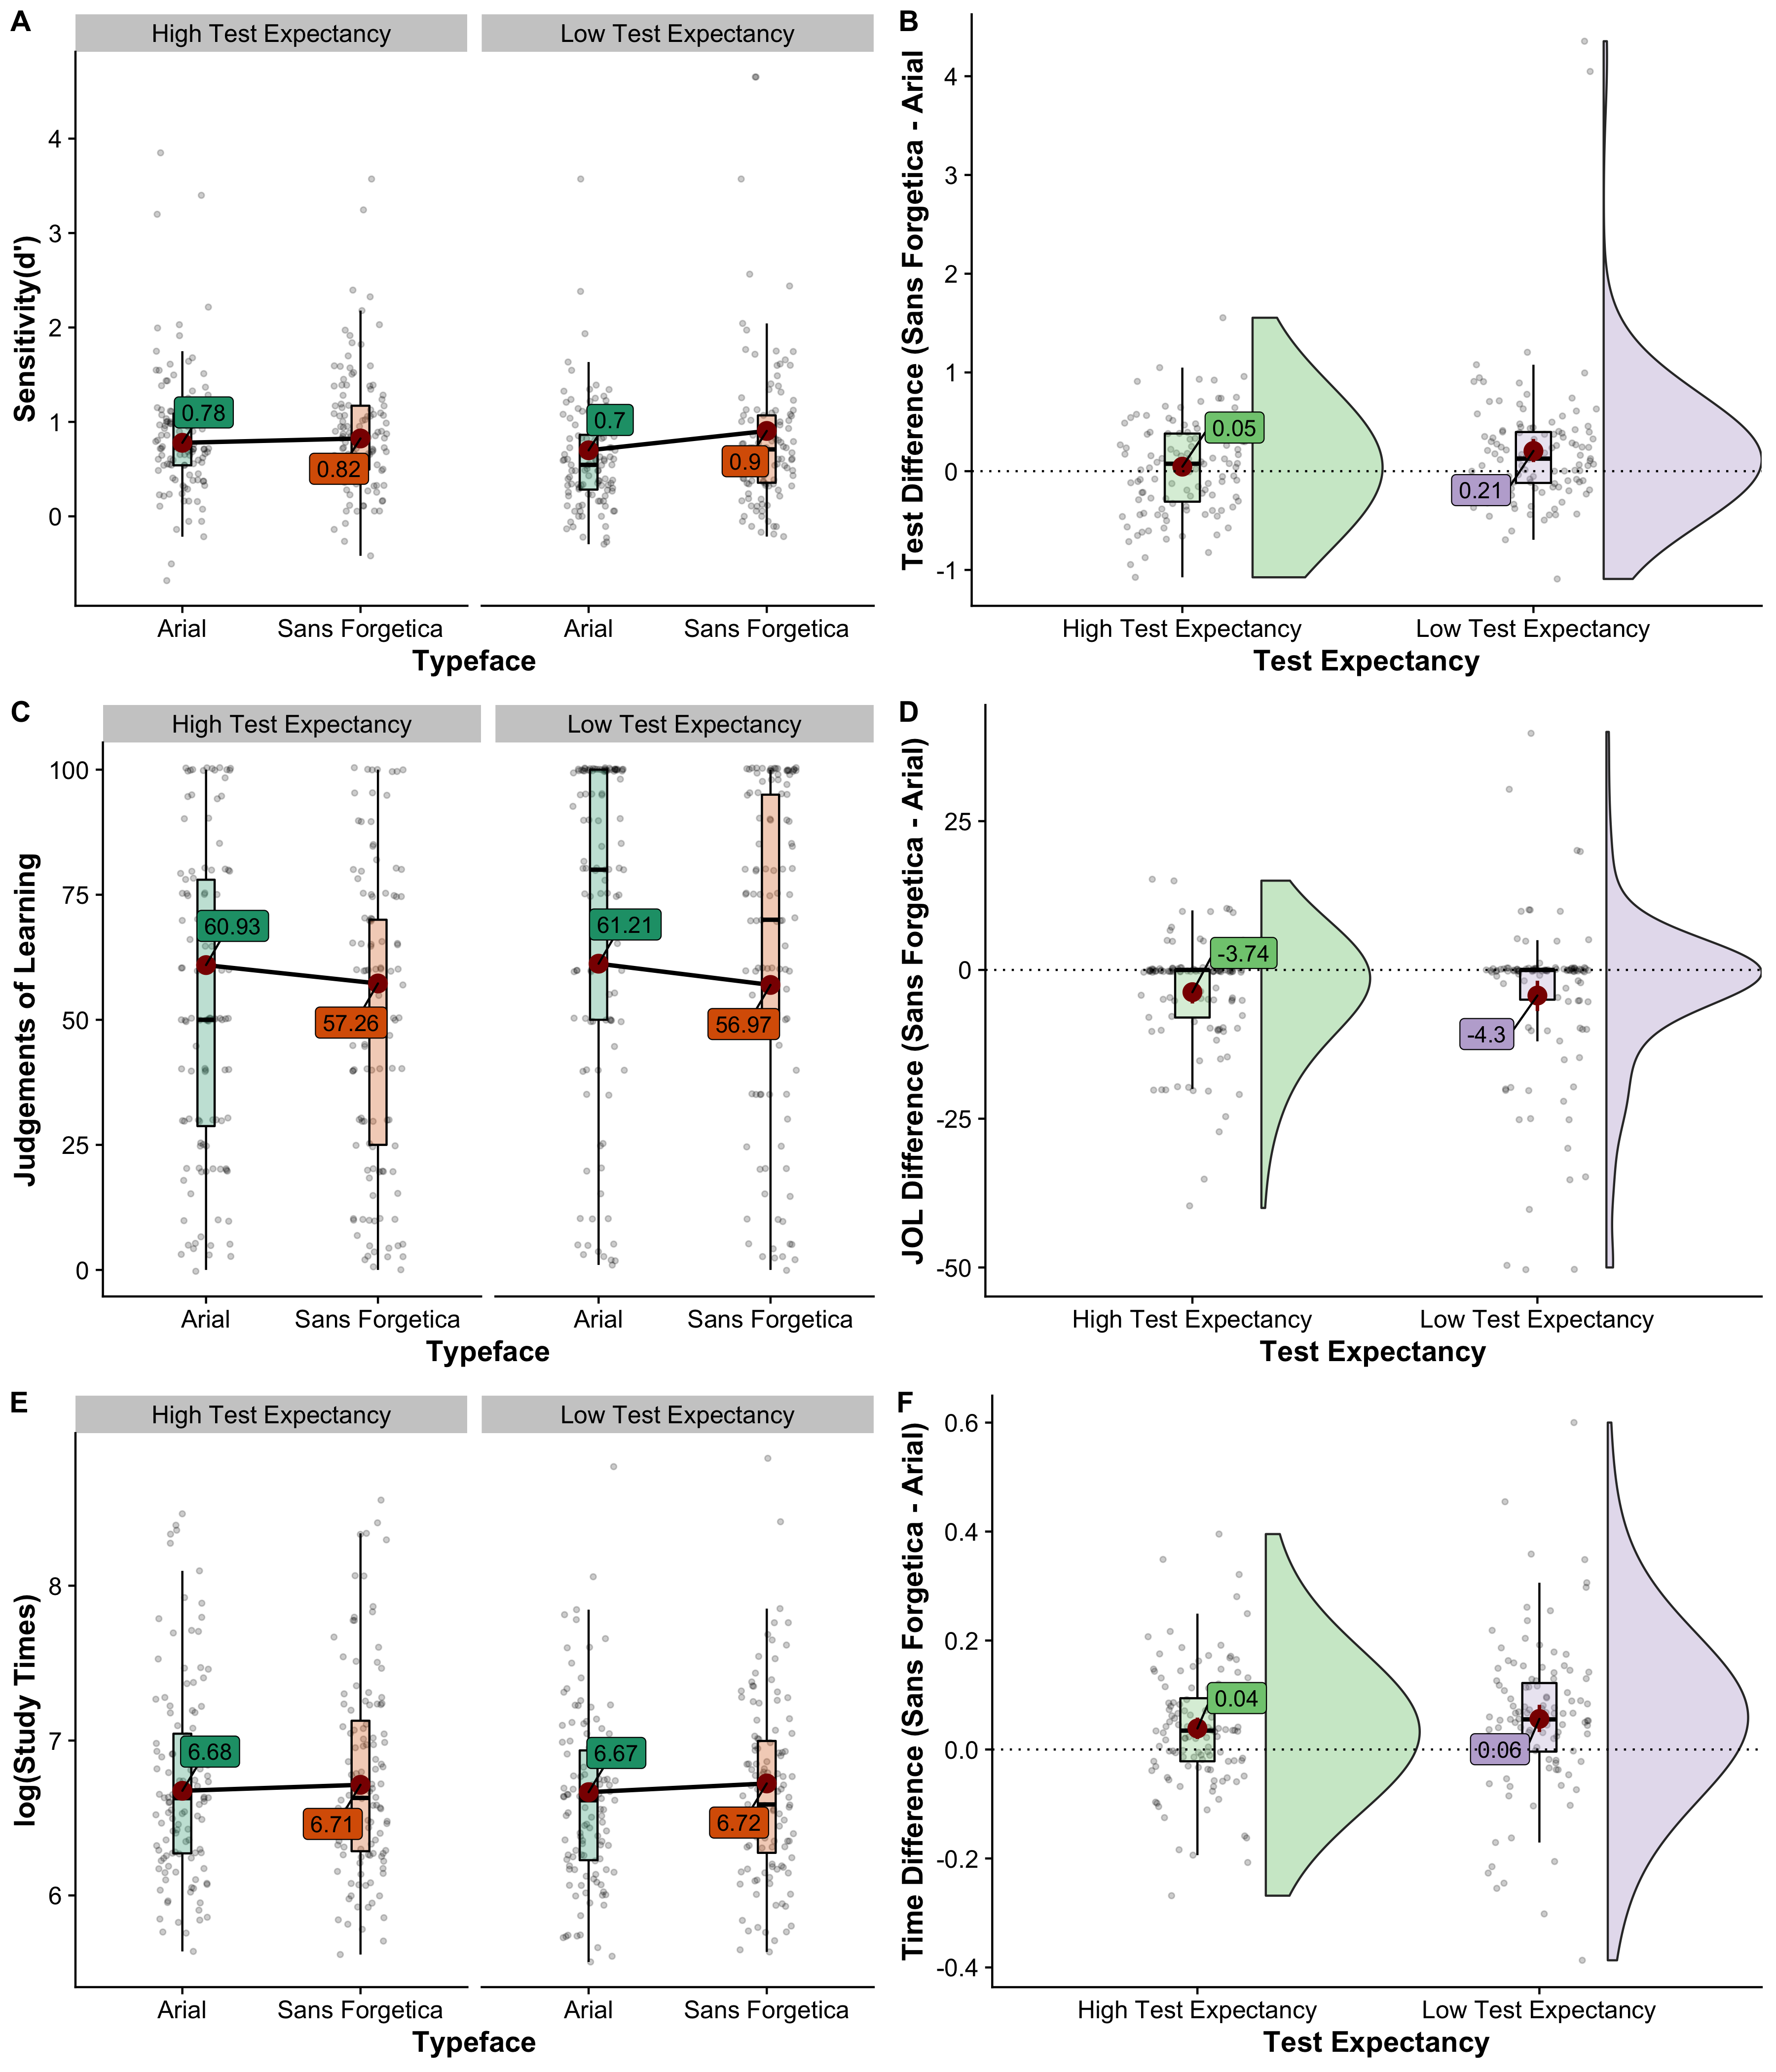
\includegraphics{Testing_Expectancy_SF_RR_files/figure-latex/unnamed-chunk-19-1} 

}

\caption{A. Participant accuracy (dots), box plots (medians and interquartile ranges), and label means for memory sensitivity (d') as a function of Typeface and Testing Expectancy in Experiment 1. B. Raincloud plots (Allen et al., 2019) for difference scores, with labeled means and bootstrapped 95\% CIs, as a function of Test Expectancy in Experiment 1. C. Participant accuracy (dots), box plots (medians and interquartile ranges), and labeled means for JOLs as a function of Typeface and Testing Expectancy in Experimenr 1. D. Raincloud plots (Allen et al., 2019) for JOL difference scores, with labeled means and bootstrapped 95\%CIs, as a function of Test Expectancy in Experiment 1. E. Participant accuracy (dots), box plots (medians and interquartile ranges), and labeled means for study times (log-transformed) as a function of Typeface and Testing Expectancy in Experiment 1. F. Raincloud plots (Allen et al., 2019) for study time difference scores, with labeled means and bootstrapped 95\% CIs, as a function of Test Expectancy in Experiment 1}\label{fig:unnamed-chunk-19}
\end{figure}

\hypertarget{experiment-2}{%
\section{Experiment 2}\label{experiment-2}}

In Experiment 2, we used weakly related cue-target pairs from Geller et al.~(2020; Experiment 1). In that experiment, participants were told about the upcoming memory test, and there was strong evidence against there being a Sans Forgetica effect (BF \textgreater{} 100). In the present experiment, we set out to examine whether this null effect persists regardless of test expectancy. That is, when test expectancy is low, will we again observe a Sans Forgetica effect with cued recall?

\hypertarget{methods}{%
\subsection{Methods}\label{methods}}

The preregistered analysis plan for Experiment 2 can be found here: \url{https://osf.io/3xak9}. All raw and summary data, materials, and R scripts for pre-processing, analysis, and plotting for Experiment 2 can be found at \url{https://osf.io/cqp6s/}.

\hypertarget{participants-1}{%
\subsubsection{Participants}\label{participants-1}}

We preregistered and collected a sample size of 232 participants. Participants were recruited on Amazon's Mechanical Turk (MTurk) platform, all of whom completed the experiment through Pavlovia (Pavolvia.org). In order to participate in the study, participants had to be native-English speakers, live in the United States, and no record of participating in previous studied offered by the researcher.

\hypertarget{design-1}{%
\subsubsection{Design}\label{design-1}}

Per our pre-registration, accuracy, JOLs, and study times were analyzed with a mixed factorial design with typeface (Arial vs.~Sans Forgetica) manipulated within-participants and test expectancy (High vs.~Low) manipulated between participants.

\hypertarget{materials-and-procedure}{%
\subsubsection{Materials and procedure}\label{materials-and-procedure}}

Materials and Procedure
Experiment 2 was programmed in PsychoPy (Peirce et al., 2019) and hosted on Pavoliva (Pavolvia.org). The materials were adopted from Geller et al.~{[}2020, Experiment 1; also see Shana K. Carpenter et al. (2006)). Participants were presented with 24 weakly related cue-target pairs. The pairs were all nouns, 5--7 letters and 1--3 syllables in length, high in concreteness (400--700), high in frequency (at least 30 per million), and had similar forward (\emph{M} = 0.031) and backward (\emph{M} = 0.033) association strengths. Two counterbalanced lists were created for each testing condition (high and low-test expectancies) so that each target could be presented in each typeface condition (Arial vs.~Sans Forgetica) without repeating any items for an individual participant.

A version of the experiment can be run by following the following link: \url{https://run.pavlovia.org/Jgeller112/sf_low_cb1}. The experiment consisted of four phases: encoding phase, JOL phase, distractor phase, and test phase. Similar to Experiment 1, some participants were told about an upcoming memory test while others were not. During the encoding phase, each participant was presented with a series of word pairs randomly, one at time with the cue always presented in Arial on the left hand side and the target word presented in either a disfluent typeface (Sans Forgetica) or a fluent typeface (Arial), on the right hand side. Typefaces of the target words were randomly intermixed. The encoding phase was self-paced: Participants were instructed to press a button of the screen after reading each word. Like Experiment 1, participants then made two list-wide JOLs. Following a short distractor task (3 min), participants were given a cued recall test which began with instructions for the test. Each trial started with the presentation of a cue from the encoding phase, in lowercase letters, to participants one at a time. Participants were instructed to type in the corresponding target (or guess if they could not remember). The test phase was self-paced. All cues were presented in Arial font. The entire experiment lasted approximately 10 minutes.

\hypertarget{scoring}{%
\subsubsection{Scoring}\label{scoring}}

Typed responses were scored with the lrd package in R (Nicholas P. Maxwell, 2020). The lrd package provides an automated way to score word responses. A partial match threshold of 80\% was used to determine whether a typed response was correct or not.

\hypertarget{results-and-discussion-1}{%
\subsection{Results and Discussion}\label{results-and-discussion-1}}

\hypertarget{cued-recall}{%
\subsubsection{Cued Recall}\label{cued-recall}}

Figures 3a shows performance in the cued-recall test (Figure 3a) along with difference scores (Figure 3b). Participants in the high test expectancy group performed better than participants in the low test expectancy group, \emph{M}\textsubscript{diff} = 20\%, \emph{F}(1, 230) = 38.26, \emph{p} \textless{} .001,\(\eta_{g}^{2}\) = .126. Participants recalled more target words in Sans Forgetica than Arial, \emph{M}\textsubscript{diff} = 5\%, \emph{F}(1, 230) = 13.57, \emph{p} \textless{} .001, \(\eta_{g}^{2}\) =.008. This was qualified by an interaction between Test Expectancy and Typeface, \emph{F}(1, 230) = 10.74, \emph{p} = .001, \(\eta_{g}^{2}\) = .006. A Bayesian analysis revealed that the interaction model was strongly preferred to the full model (BF = 21.77). Planned comparisons showed that individuals in the low test expectancy group recalled more words presented in Sans Forgetica than Arial, \emph{t} =4.92, \emph{p} \textless{} .001, \emph{d}\textsubscript{avg}= 0.38; In the high test expectancy group, there was substantial evidence that there was no difference between Sans Forgetica and Arial, \emph{t} = 0.287, \emph{p} = .778, \emph{d}\textsubscript{avg} = 0.02, BF\textsubscript{01} = 9.31.

\hypertarget{jols-1}{%
\subsubsection{JOLs}\label{jols-1}}

Figures 3c and 3d show JOLs (Figure 3b) as well as difference scores (Figure 4c). Using the same model as above, participants in the high test expectancy group gave higher JOLs than the low test expectancy group, \emph{M}\textsubscript{diff} = 5.91, \emph{F}(1,229) = 13.57, \emph{p} \textless{} .001, \(\eta_{g}^{2}\) = .028. Arial elicited higher JOLs than Sans Forgetica, \emph{M}\textsubscript{diff} = 15.15, \emph{F}(1,229) = 87.05, \emph{p} \textless{} .001, \(\eta_{g}^{2}\) = .161. There was an interaction between Testing Expectancy and Typeface, \emph{F}(1,229) = 13.65, \emph{p} \textless{} .001, \(\eta_{g}^{2}\) \textless{} .029. A Bayesian analysis revealed that the interaction model was strongly preferred to the main effects-only model (BF \textgreater{} 100). Planned comparisons revealed that the JOL effect was larger in the low test expectancy group (\emph{d}\textsubscript{avg} = 1.21) than in the high test expectancy group (\emph{d}\textsubscript{avg} = 0.72).

\hypertarget{study-times-1}{%
\subsubsection{Study Times}\label{study-times-1}}

Figures 3e and 3f show log-transformed RTs (Figure 3e) and difference scores (Figure 4f). Like Experiment 1, we excluded study times less than 150 ms and study times greater than 2.5 SD above the mean per condition for each participant. The outlier procedure removed \textasciitilde{} 2\% of the data. Study times were overall larger for the high test expectancy group compared to the low test expectancy group, \emph{M}\textsubscript{diff} = 0.34, \emph{F}(1,230) = 17.02, \emph{p} \textless{} .001, \(\eta_{g}^{2}\) = .068. Cue-target pairs yielded larger study times for Sans Forgetica compared to Arial, \emph{M}\textsubscript{diff} = 0.06, \emph{F}(1,230) = 27.74, \emph{p} \textless{} .001, \(\eta_{g}^{2}\) = .002. There was no interaction between Testing Expectancy and Typeface, F(1,230) = 0.39, \emph{p} = .533, \(\eta_{g}^{2}\) \textless{} .001. A main effects-only model was strongly preferred over the interaction model (BF = 6.03).

\hypertarget{jol}{%
\subsection{JOL}\label{jol}}

\hypertarget{rts}{%
\subsection{RTs}\label{rts}}

\begin{figure}

{\centering 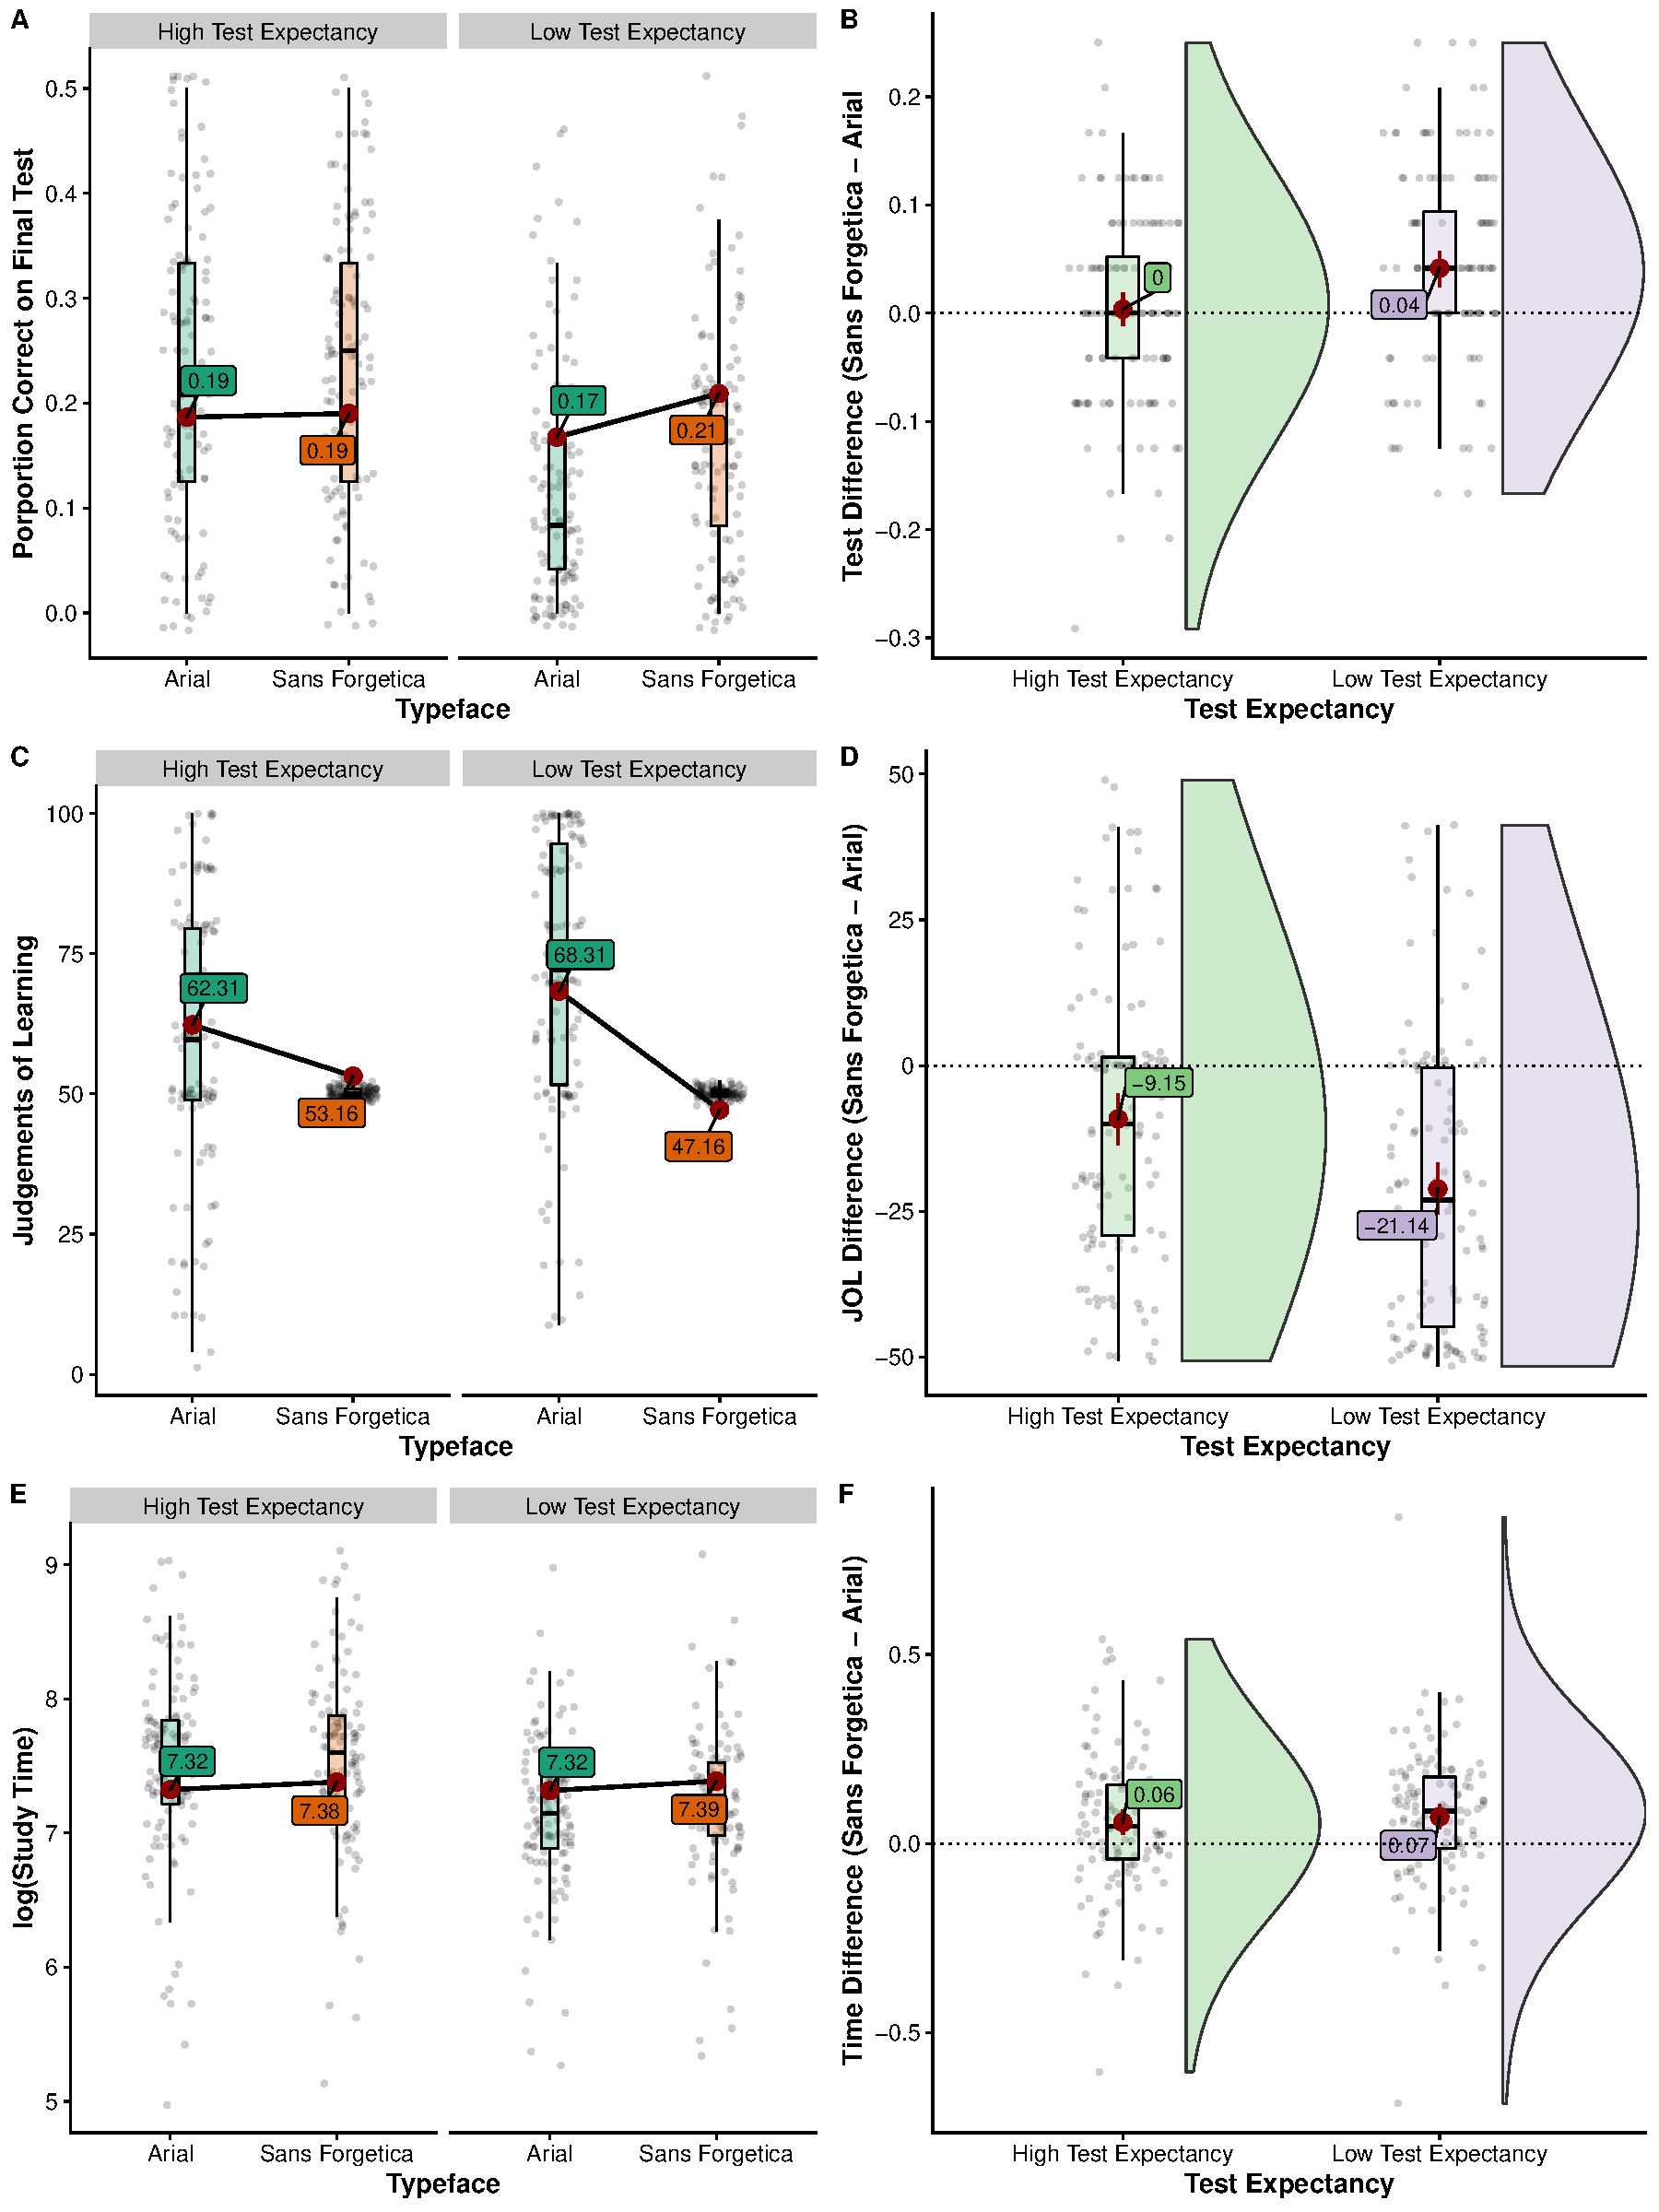
\includegraphics{Testing_Expectancy_SF_RR_files/figure-latex/unnamed-chunk-56-1} 

}

\caption{ }\label{fig:unnamed-chunk-56}
\end{figure}

The results complement those from Experiment 1 well and suggest the disfluency effect with Sans Forgetica is not unique to a particular criterion test. Using cued recall, we once again demonstrated that Sans Forgetica can constitute a desirable difficulty, but only when test expectancy is low. Importantly, the effect we observed was rather modest; Sans Forgetica conferred roughly a 5\% increase in cued recall performance above and beyond Arial, a more fluent typeface. When looking at the low test expectancy group alone we observed a 9\% increase. Furthermore, we once again showed longer study times and lower JOLs for words studied in Sans Forgetica. There are, however, a couple points of divergence that merit mention. Compared to Experiment 1, JOLs for the Sans Forgetica condition were tightly bunched around the middle of the response scale.\footnote{Experiments 2 and 3 used a slider scale that ranged from 0-100 in increments of 10 while Experiment 1 had participants type in a number between 0-100.} This could reflect uncertainty around how well participants remember Sans Forgetica target words. Additionally, study times for Sans Forgetica were longer for the high test expectancy group compared to the low test expectancy group. This most likely reflects participants studying word pairs longer in preparation for an upcoming test.

\hypertarget{experiment-3}{%
\section{Experiment 3}\label{experiment-3}}

In Experiments 1 and 2, we observed a benefit for Sans Forgetica under low test expectancy. Although this result constitutes an example of a desirable difficulty effect as a result of perceptual disfluency, the mechanisms underlying such effects remain an open issue. Our preferred interpretation is that encoding difficulty from the typeface is an attentional response eliciting deeper processing that in turn leads to better remembering. However, another possible explanation is that Sans Forgetica is remembered better simply because participants spend more time processing them, as indexed by slower study times during encoding in both Experiments 1 and 2.\footnote{A simple time-on-task account does a poor job of explaining the lack of a Sans Forgetica effect we observed in Experiments 1 and 2 when participants were told about a memory test.}.

To examine if time-on-task can account for the desirable effect of Sans Forgetica on recall, we manipulated time spent encoding by having participants either encode stimuli at their own pace (self-paced), or by removing control over how long the stimuli were studied for. If time-on-task moderates the Sans Forgetica effect, we expect there to be no effect on memory when time is constrained to be equal between Arial and Sans Forgetica. However, when encoding is self-paced, we would expect there to be better memory for Sans Forgetica compared to Arial. Corroborating this, Kühl et al. (2014) showed that self-paced study produced better learning outcomes compared to constrained study time. Because of this, we hypothesized that we would observe a disfluency effect for Sans Forgetica only when study time was self-paced.

In Experiment 3 we choose to keep testing expectancy low and manipulate time-on-task (self-paced vs.~3 s)\footnote{Three seconds was chosen by looking at overall study times for Experiment 2 (M = 2,192 ms). Given this, we thought 3 s would be more than sufficient to allow identification of the cue-target pairs}. This design also served to replicate the novel findings from Experiment 2 showing that low test expectancy is essential for the Sans Forgetica memory effect. In addition, we examine list-wide JOLs. Due to the experiment design, we could not analyze study times as they could only be collected in the self-paced group.

\hypertarget{methods-1}{%
\subsection{Methods}\label{methods-1}}

The preregistration for this experiment can be found here: \url{https://osf.io/hjnk5}. All raw and summary data, materials, and R scripts for pre-processing, analysis, and plotting for Experiment 3 can be found at \url{https://osf.io/cqp6s/}.

\hypertarget{participants-2}{%
\subsubsection{Participants}\label{participants-2}}

We preregistered and collected a sample size of 232 participants. Participants were recruited on Prolific , all of whom completed the experiment through Pavlovia (Pavolvia.org). Using prescreening questionnaires on Prolific, we limited our sample to participants to those residing in the USA, native English speakers, and had no record of participating in previous studies by the first author.

\hypertarget{design-materials-and-procedure}{%
\subsubsection{Design, Materials, and Procedure}\label{design-materials-and-procedure}}

The design, materials, and procedure are identical to Experiment 2, with one exception---instead of manipulating test expectancy (no participants were informed of the impending memory test in Experiment 3), study time was manipulated (Self-paced vs.~3 s) between participants. In the self-paced group (like in Experiment 2), participants were given as long as they wanted to process the cue-target pairs. In the 3 s group, cue-target pairs were presented for 3 seconds.

\hypertarget{results-and-discussion-2}{%
\subsection{Results and Discussion}\label{results-and-discussion-2}}

\hypertarget{cued-recall-1}{%
\subsubsection{Cued Recall}\label{cued-recall-1}}

Figures 4a shows performance on the cued recall test (Fig. 4a) along with difference scores (Figure 4b). The analysis revealed that there was no reliable difference between the Self-paced and Timed groups on cued recall, \emph{M}\textsubscript{diff} = 2\%, \emph{F}(1, 230) = 0.369, \emph{p} \textless{} .544, \(\eta_{g}^{2}\) = .055. Individuals were better at recalling target words presented in Sans Forgetica than Arial, \emph{M}\textsubscript{diff} = 5\%, \emph{F}(1, 230) = 15.03, \emph{p} \textless{} .001, \(\eta_{g}^{2}\) =.013. This was no interaction between Time on Task and Typeface, \emph{F}(1, 230) = 1.13,\emph{p} = .289, \(\eta_{g}^{2}\) \textless{} .001. A Bayesian analysis revealed that a main effects-only model was preferred to the interaction (BF = 5.50).

\hypertarget{jols-2}{%
\subsection{JOLs}\label{jols-2}}

Figure 4c shows JOLs (Figure 4c) and difference scores (Fig 4d). Using the same model as above, participants in the Timed group gave higher JOLs than in the Self-paced group, \emph{M}\textsubscript{diff} = 5.91, \emph{F}(1,230) = 17.43, \emph{p} \textless{} .001, \(\eta_{g}^{2}\) = .055. Arial typeface elicited higher JOLs than Sans Forgetica typeface, \emph{M}\textsubscript{diff} = 9.7, F(1,230) = 48.81, p \textless{} .001, \(\eta_{g}^{2}\) = .048. There was an interaction between Time on Task and Typeface, \emph{F}(1,230) = 27.17, \emph{p} \textless{} .001, \(\eta_{g}^{2}\) \textless{} .027. A Bayesian analysis revealed that the interaction model was strongly preferred to the main effects-only model (BF = 57.24). Simple effects revealed that the JOL effect (Arial \textless{} Sans Forgetica) was larger in the self-paced group (\emph{d}\textsubscript{avg} = 1.22) than in the timed group (\emph{d}\textsubscript{avg} = 0.10; BF\textsubscript{01} = 1.466).

Taken together, the results from Experiment 3 are clear. Cued recall performance was better overall for Sans Forgetica---it did not matter if encoding was self-paced or timed. This contradicts a study by Kühl et al.~(2014) showing that self-paced study produces better learning outcomes compared to constrained study time. It is important to note that our study used simple learning materials whereas Kühl et al., used more complex materials (i.e., multimedia slides about lightening construction). With more complex materials, a time limit might hurt rather than help recall. Despite this, the findings from Experiment 3 nicely replicated the findings from Experiment 2 under low test expectancy. From this, it is clear that a simple time-on-task account cannot explain these findings. A time on task account would predict better memory in the self-paced group because they can spend longer encoding each pair. While the interaction was not significant, looking at the effect sizes between groups, the disfluency effect was larger in the timed group (\emph{d}\textsubscript{avg} = 0.32) than the self-paced group (\emph{d}\textsubscript{avg} = 0.15). We return to this issue in the general discussion.

\begin{figure}

{\centering 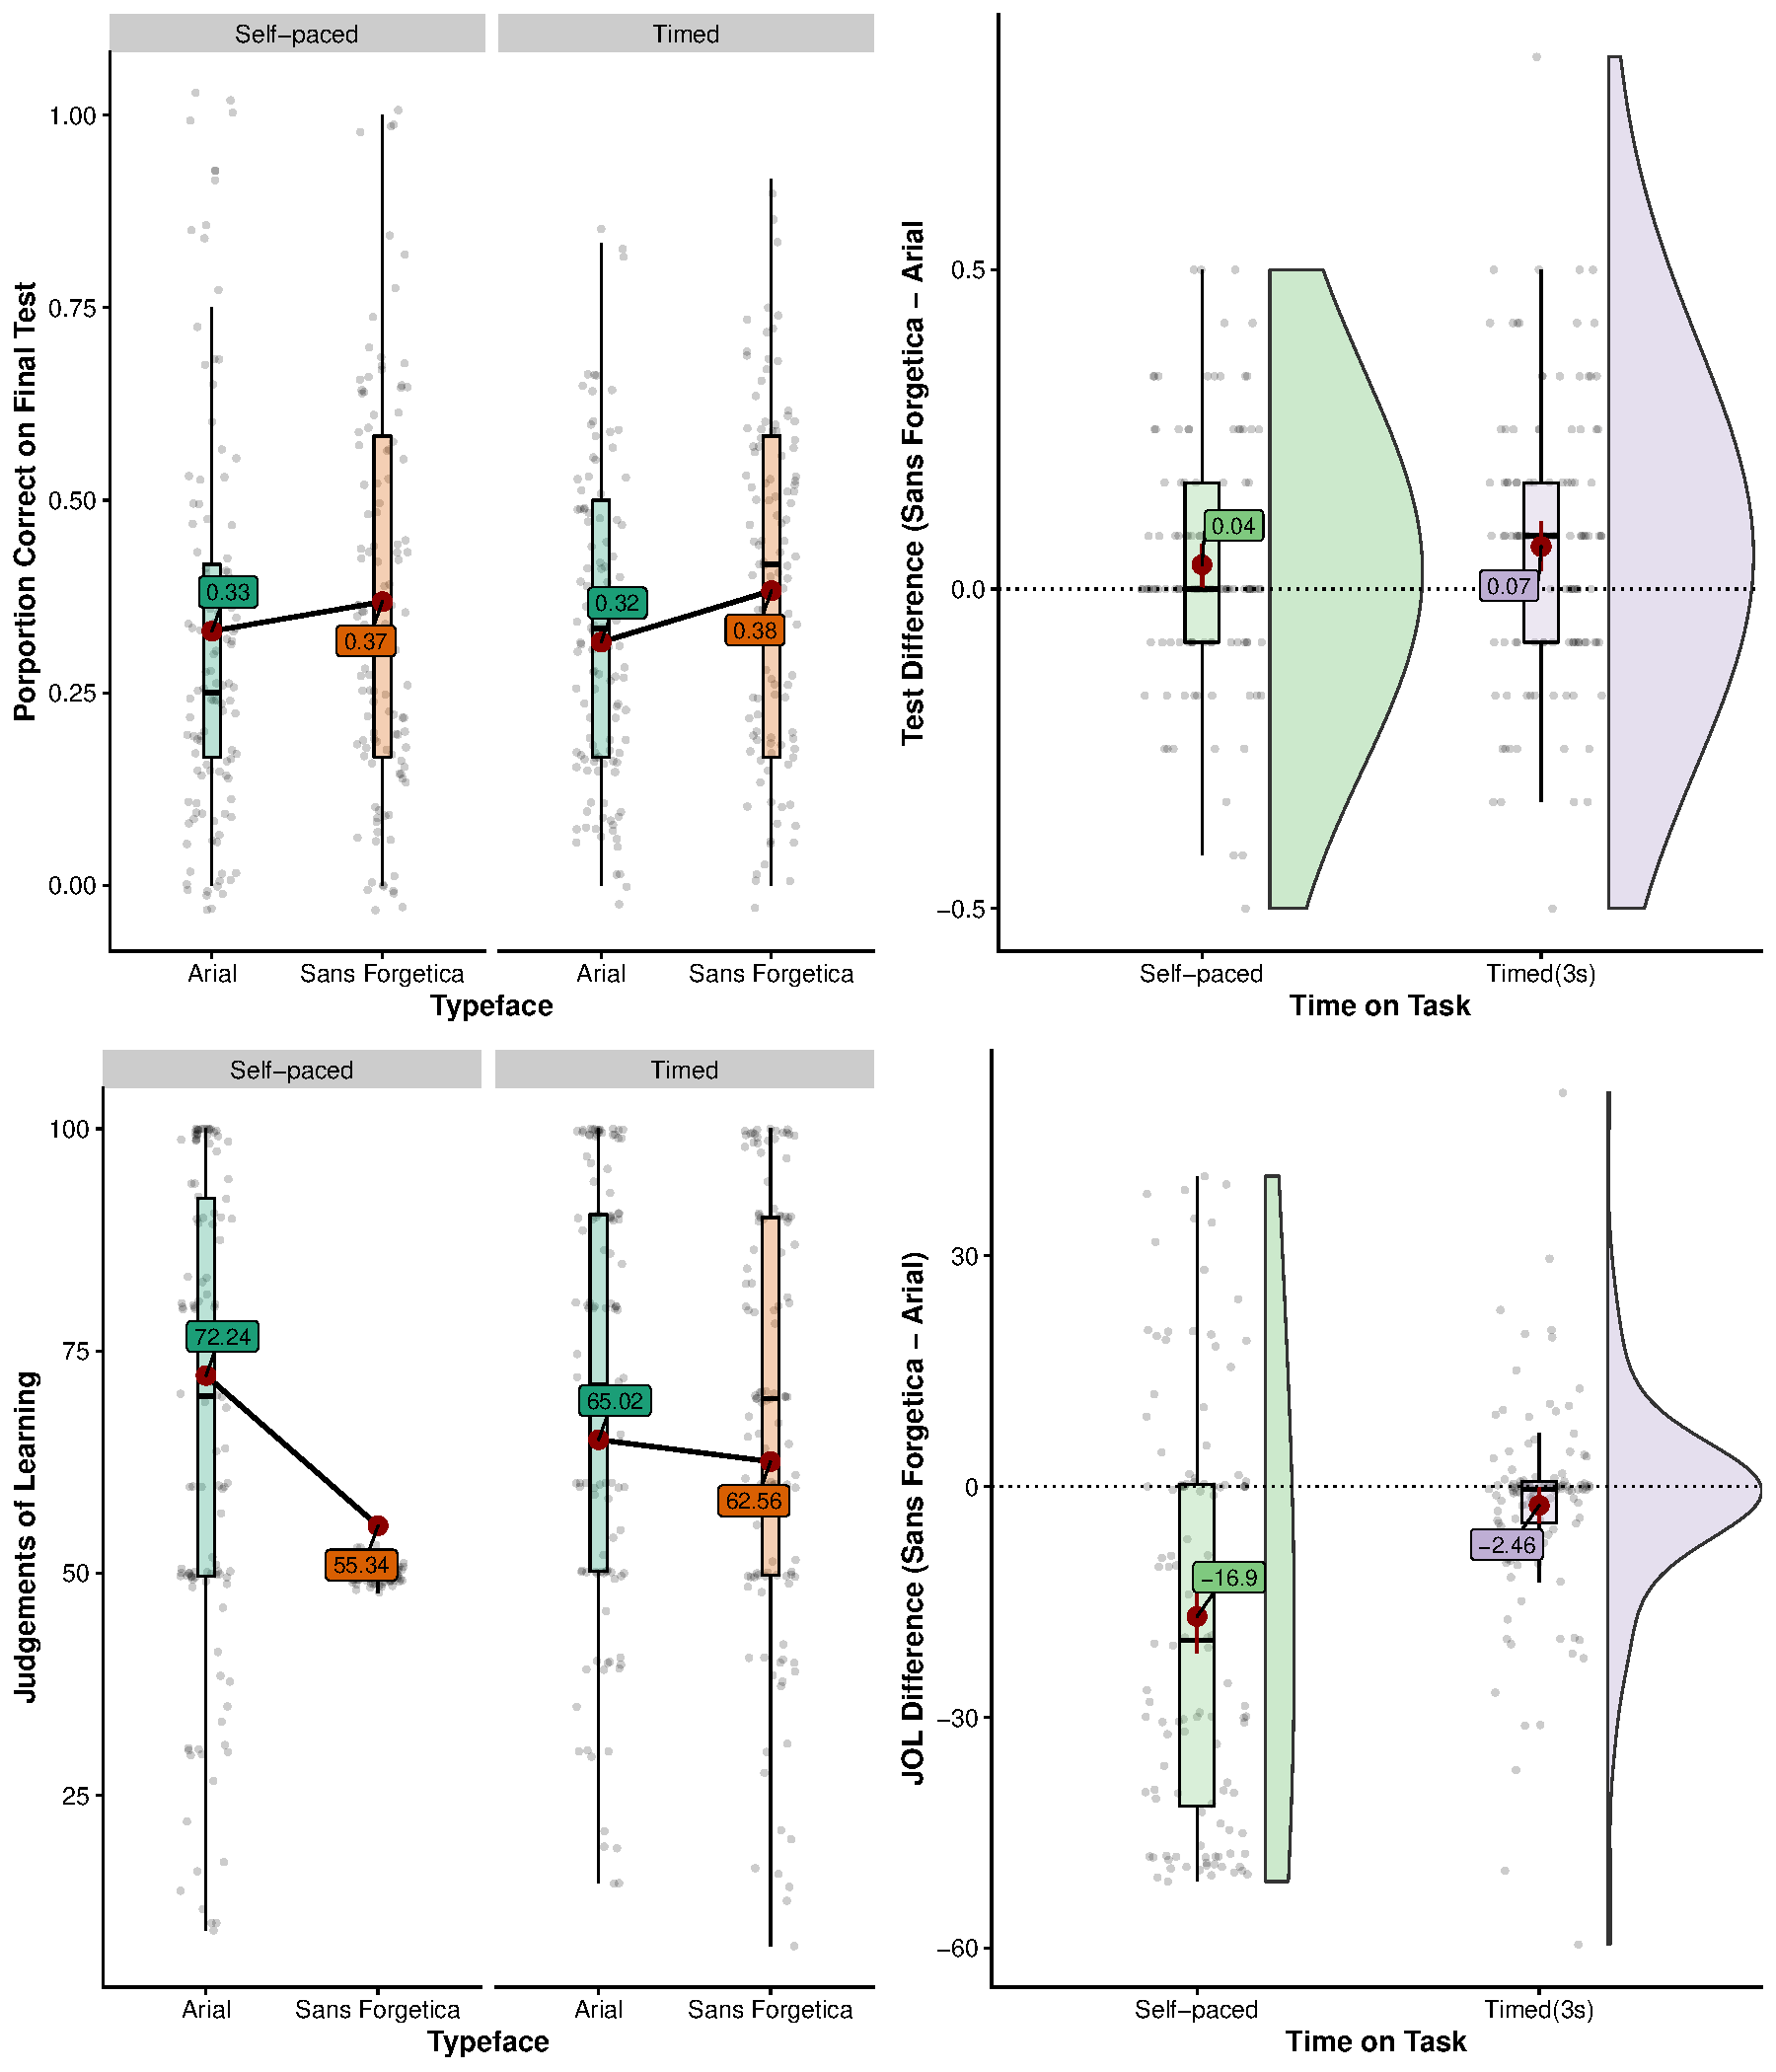
\includegraphics{Testing_Expectancy_SF_RR_files/figure-latex/unnamed-chunk-74-1} 

}

\caption{A. Participant accuracy (dots), box plots (with medians and interquartile ranges), and labeled means for cued recall as a function of Typeface and Time-on-Task in Experiment 3. B. Raincloud plots (Allen et al., 2019) for cued recall difference scores, with labeled means and bootstrapped 95\% CIs, as a function of Time-on-Task in Experiment 3. C. Participant accuracy (dots), box plots (with medians and interquartile ranges), and labeled means for JOLs as a function of Typeface and Time-on-Task in Experiment 3. D. Raincloud plots (Allen et al., 2019) for JOL difference scores, with labeled means and bootstrapped 95\% CIs as a function of Time-on-Task in Experiment 3}\label{fig:unnamed-chunk-74}
\end{figure}

Turning to JOLs, we replicated the outcomes from Experiments 1 and 2 showing that participants judged Sans Forgetica as less memorable (lower JOLs). This difference was larger in the self-paced group than in the timed group. While the reason for this is not clear, one possible explanation could be that during self-paced encoding, individuals are more uncertain about whether they will remember disfluent targets because they were not restricted by a time limit and could advance at their own pace. This fact is highlighted by JOLs in that condition clustering around the middle point of the scale.

\hypertarget{general-discussion}{%
\section{General Discussion}\label{general-discussion}}

Sans Forgetica has garnered substantial attention from both the media and the scientific community as of late. The present experiments attempted to reconcile the mixed findings in the literature as it relates to Sans Forgetica and more broadly, perceptual disfluency. Following up on recent calls to examine boundary conditions of the perceptual disfluency effect (R. A. Bjork \& Yue, 2016; Dunlosky \& Mueller, 2016), we focused on one boundary condition: testing expectancy. To summarize, we found evidence that testing expectancy moderates the perceptual disfluency effect. Sans Forgetica produced lower JOLs and longer study times across (Experiments 1 and 2) and enhanced memory in recognition (Experiment 1) and cued recall (Experiment 2) only when participants were not told an upcoming memory test. Experiment 3 revealed this effect does not seem to be a solely mediated by time-on-task.

These outcomes conflict with some recent findings. First, Rosner et al.~(2015, experiment, 3A) did not find a moderating role for test expectancy in recognition memory using a high-level blurring manipulation---low and high test expectancy elicited a similar benefit. Despite this, those findings have not been replicated, closely or conceptually. In the current set of experiments, we demonstrated a robust effect of test expectancy across different test formats (Experiments 1 and 2), and replicated the basic disfluency effect with low test expectancy (Experiment 3). One interesting possibility is that disfluency manipulations can have differential effects on memory. For instance, in Rosner et al., (2015; Experiment 4a), they were only able to show a desirable effect of blurring using a high-level blurring manipulation---they could not find a recognition benefit using a low-level blurring manipulation. Similarly, Geller et al.~(2018) showed that easy-to-read cursive words produced stronger memory effects than hard-to-read cursive words. Thus, the blurring manipulation used by Rosner et al.~might have been a stronger cue than Sans Forgetica. An important avenue for future research would be examine different levels and types of perceptual disfluency and their role on memory.

Additionally, while we found a general benefit of Sans Forgetica under low test expectancy, Eskenazi and Nix (2020) only found a memory benefit for Sans Forgetica among those participants who were stronger spellers. Better spellers are thought to have a more precise mental lexicon which allows for more efficient processing at multiple levels of representation (i.e., orthographic, phonological, and semantic; Perfetti, 2007). When confronted with perceptual degradation, better spellers would be able to process a stimulus at a deeper level, which could give rise to better memory. The disparate findings can be reconciled by the fact that we used high frequency words in all three experiments. Presumably, these words were well known to the participant therefore allowing perceptual disfluency to be desirable for learning.

\hypertarget{perceptual-desirable-difficulty-a-time-on-task-effect}{%
\subsection{Perceptual Desirable Difficulty: A Time on Task Effect?}\label{perceptual-desirable-difficulty-a-time-on-task-effect}}

The result of primary interest here is that Sans Forgetica, a perceptually disfluent typeface, was associated with better recognition and recall, but only when test expectancy was low. It has been proposed that perceptual disfluency enhances memory as a result of deeper, more effortful, processing. A rather uninteresting alternative explanation is that an extended period of time dedicated to encoding is sufficient to enhance memory encoding. While a time on task account can explain the Sans Forgetica effect under low test expectancy, it is not adequate to explain some of the other findings. In both Experiments 1 and 2, Sans Forgetica produced longer study times, yet there was strong evidence that there was no perceptual disfluency effect in the high test expectancy group. Furthermore, in Experiment 3, where we directly tested time-on-task by having participants either encode cue-target pairs with a time-limit, or have encoding be self-paced, we found robust effects of perceptual disfluency on cued recall regardless of pacing. In addition, we found that the perceptual disfluency effect were larger under a time constraint than it was when encoding was self-paced. It is not clear how a time-on-task account would explain these findings.

In addition, a simple time-on-task account has been refuted in other studies. In Geller et al.~(2018), for example, the authors showed that while hard-to-read cursive words engendered longer naming latencies, they did not enhance memory at test compared to an easy-to-read cursive manipulation. Similarly, Rosner et al.~(2015), showed that while a low-level blurring condition produced longer naming latencies, it did not enhance memory at test . In contrast, a higher level of perceptual blur slowed naming latencies and enhanced recognition memory at test. These results suggest that perceptual degradation affects naming times in the study phase in a continuous manner, but that perceptual degradation at study must surpass some threshold to induce processing that enhances memory encoding.

\hypertarget{theoretical-mechanisms-of-the-perceptual-disfluency-effect}{%
\subsection{Theoretical Mechanisms of the Perceptual Disfluency Effect}\label{theoretical-mechanisms-of-the-perceptual-disfluency-effect}}

If perceptual disfluency is not driven by time-on-task, what then? The current findings add to our understanding of the mechanism(s) underlying the desirable effects of perceptual disfluency on memory. Eitel and Kühl (2016) postulated that if Sans Forgetica is a desirable difficulty, it fosters learning by increasing mental effort and by stimulating deeper processing. When preparing for an upcoming test (high testing expectancy), there is a high investment of effort allocated to the material, regardless of whether the to-be-learned information is fluent or disfluent---which would attenuate the effects of disfluency. Looking at both testing expectancy groups (see Figures 2b and 3b), there is some evidence for this. In both groups, recognition memory and cued recall was generally higher for Sans Forgetica, suggesting those stimuli received deeper processing, while the processing of Arial words appear to be shallower in the low test expectancy group. This suggests that with high test expectancy all words get deeper processing resulting in a smaller difference in the high test expectancy group.

Given that high testing expectancy eradicated the mnemonic benefit of Sans Forgetica, this points to a similar mechanism of action---that is, deeper, more effortful, processing at encoding. Just how this processing is carried out is still subject to debate. Geller et al.~(2018) recently provided a potential answer to this question. They presented participants with varying levels of handwritten cursive stimuli (easy-to-read and hard-to-read) in order to adjudicate between current accounts of perpetual disfluency (i.e., metacognitive and compensatory processing accounts). From a metacognitive perspective, the memory benefit should be equal for easy-to-read and hard-to-read cursive words---within that account, all disfluency types are created equal (Weissgerber et al., 2017). However, the compensatory processing account suggests that the memory benefit should be greater for hard-to-read cursive stimuli. This is because during word identification hard-to-read cursive are harder and therefore should elicit more lexical/semantic processing (Perea et al., 2016). In contrast to both accounts, Geller et al.~found that easy-to-read cursive were better remembered than hard-to-read cursive words, despite not being as hard. This pattern is hard for extant accounts to explain. This prompted Geller et al.~to propose an alternative explanation for disfluency effects. Within their account, perceptual disfluency effects arise due to (1) increased processing difficulty during recognition (i.e., difficulty mapping letters to words) and (2) deeper processing that occurs after recognition, presumably as the result of some combination of semantic processing and metacognitive control and regulatory components. This account can explain the lack of disfluency effect in the high test expectancy group as a result of increased metacognitive monitoring and control processes eliciting attention to both types of stimuli.

A more general framework that invokes cognitive monitoring and control, such as the conflict monitoring framework (Botvinick et al., 2001), might also explain the present findings (see Geller et al., 2018; Rosner et al., 2015). Within this framework, the up- and down-regulation of monitoring and control are mediated by response ambiguity or conflict (in the current case, difficulty identifying the word). Under low test expectancy, Sans Forgetica would trigger greater control due to the difficulty associated with recognizing the stimulus---this serves to enhance memory. However, under high testing expectancy, the goal is switched to remember words for an upcoming memory test, and while Sans Forgetica is still harder, monitoring and control processes are directed to both types of stimuli, dampening/weakening the disfluency effect. The exact mechanisms underlying perceptual disfluency remain an open issue and more research is needed to better understand how perceptual disfluency enacts a desirable effect on memory.

\hypertarget{practical-implications}{%
\subsection{Practical Implications}\label{practical-implications}}

The current findings have some educational significance. While it might be tempting to conclude from these findings that Sans Forgetica should be used as study tool, the current results need to be interpreted with caution. First, and most importantly, the conclusion that Sans Forgetica is only beneficial to memory under low test expectancy makes its use in the educational domain impractical. In the classroom, students rarely encode information incidentally; learning is always purposeful and goal directed. Second, the experimental paradigms used involved simple list learning. It is not clear if Sans Forgetica would benefit learning under low test expectancy with more complex materials. Some evidence from Taylor et al.~(2020, Experiments 3 and 4) suggests it might not. In those experiments, memory for factual and conceptual information was tested using more educationally realistic materials (prose passages) and displayed no mnemonic advantage for Sans Forgetica. Thus, even with low testing expectancy, Sans Forgetica did not enhance memory when the to-be-learned material was more educationally realistic.
Second, the effect sizes from all three experiments were rather modest by conventional standards Funder \& Ozer (2019) (Experiment 1 - \emph{d}\textsubscript{avg} = 0.31; Experiment 2 - \emph{d}\textsubscript{avg} = 0.38; Experiment 3 - Timed: \emph{d}\textsubscript{avg} = 0.32; Self-paced: \emph{d}\textsubscript{avg} = 0.15). It is unclear if the Sans Forgetica effect would replicate in educational settings where effect sizes are a known to be a smaller and more variable (Butler et al., 2014).

Finally, there is a fair amount of variability in the number of participants that benefited from perceptually disfluency. If you look at the difference scores presented in Figures 2, 3, and 4, positive effects are not seen consistently. In fact, some students are hurt by the presentation of Sans Forgetica. Before we start recommending perceptual disfluency as a potential study tool, it is critical we better understand the nature of these individual differences (i.e., why perceptual disfluency hurts some students while benefiting others).

We do acknowledge, however, that Sans Forgetica might have some practical implications. Outside the classroom, information is largely acquired incidentally, without the goal of memorization (Castel et al., 2015). If this is the case, information presented in Sans Forgetica might serve to indirectly enhance memory. For instance, one area where perceptual disfluency might be desirable is in advertising. We acquire visual information, incidentally, via billboards, online advertisements, magazines, etc. Placing this type of information in a perceptually disfluent typeface like Sans Forgetica might be helpful. However, before any definitive claims are made we need to have a better understanding of the conditions under perceptual disfluency is and is not desirable for learning.

\hypertarget{conclusions}{%
\subsection{Conclusions}\label{conclusions}}

Recent reports have recommended that teachers and students use perceptual disfluency to enhance learning. Although we have shown that a simple perceptual manipulation (i.e., placing material in Sans Forgetica) can enhance learning in a very simplified context (i.e., list learning), its efficacy as a potential learning technique is tempered by the finding that testing expectancy can nullify the effect. In educational settings, learning is explicitly goal-directed, and students accordingly encode information intentionally. Thus, Sans Forgetica (and perceptual disfluency manipulations in general) may not effectively enhance memory in ecologically valid settings. While a recent meta-analysis (H. Xie et al., 2018) claimed the disfluency effect was null and void, what is clear from the current findings is that the impact of perceptual disfluency manipulations such as Sans Forgetica, is not straightforward. Researchers should heed the call to further examine the conditions under which perceptual disfluency is and not desirable for learning.

\newpage

\hypertarget{disclosures}{%
\subsection{Disclosures}\label{disclosures}}

\hypertarget{acknowledgements}{%
\subsubsection{Acknowledgements}\label{acknowledgements}}

This research was supported by grant number 220020429 from the James S. McDonnell Foundation awarded to the second author. We would like to Gene Brewer and two anonymous reviewers for their helpful comments on an earlier draft of the paper.

\hypertarget{conflicts-of-interest}{%
\subsubsection{Conflicts of Interest}\label{conflicts-of-interest}}

The authors declare that they have no conflicts of interest with respect to the authorship or the publication of this article.
\newline

\hypertarget{author-contributions}{%
\subsubsection{Author Contributions}\label{author-contributions}}

JG wrote the manuscript, collected data, and conducted all statistical analyses.DJP edited the manuscript and provided feedback.
\newline

\hypertarget{r-and-r-package-acknowledgements}{%
\subsubsection{R and R package acknowledgements}\label{r-and-r-package-acknowledgements}}

This paper was written in R-Markdown. In RMarkdown, the text and the code for analysis may
be included in a single document. The document for this paper, with all text and code, can be found at: . The results were created using R (Version 4.0.2; R Core Team, 2019) and the R-packages \emph{afex} (Version 0.27.2; Singmann et al., 2019), \emph{BayesFactor} (Version 0.9.12.4.2; Morey \& Rouder, 2018b), \emph{carData} (Version 3.0.4; Fox et al., 2019), \emph{coda} (Version 0.19.3; Plummer et al., 2006), \emph{cowplot} (Version 1.1.0; Wilke, 2020), \emph{data.table} (Version 1.13.0; Dowle \& Srinivasan, 2020), \emph{dplyr} (Version 1.0.3; Wickham et al., 2019), \emph{effects} (Fox, 2003; Fox \& Hong, 2009; Version 4.2.0; Fox \& Weisberg, 2018), \emph{emmeans} (Version 1.5.0; Lenth, 2020), \emph{forcats} (Version 0.5.0; Wickham, 2019a), \emph{ggplot2} (Version 3.3.2; Wickham, 2016b), \emph{ggpol} (Version 0.0.6; Tiedemann, 2019), \emph{ggrepel} (Version 0.8.2; Slowikowski, 2020), \emph{here} (Version 0.1; Müller, 2017), \emph{janitor} (Version 2.0.1; Firke, 2020), \emph{knitr} (Version 1.31; Y. Xie, 2015), \emph{lattice} (Version 0.20.41; Sarkar, 2008), \emph{lme4} (Version 1.1.25; Bates et al., 2015), \emph{lubridate} (Version 1.7.9; Grolemund \& Wickham, 2011), \emph{Matrix} (Version 1.2.18; Bates \& Maechler, 2019), \emph{modelbased} (Version 0.4.0; Makowski et al., 2020), \emph{MOTE} (Version 1.0.2; Buchanan, Gillenwaters, et al., 2019), \emph{papaja} (Version 0.1.0.9997; Aust \& Barth, 2020), \emph{patchwork} (Version 1.1.0; Pedersen, 2019), \emph{plyr} (Wickham, 2011; Version 1.8.6; Wickham et al., 2019), \emph{purrr} (Version 0.3.4; Henry \& Wickham, 2019), \emph{qualtRics} (Version 3.1.3; Ginn \& Silge, 2020), \emph{readr} (Version 1.3.1; Wickham et al., 2018), \emph{report} (Version 0.2.0; Makowski et al., 2020), \emph{Rmisc} (Version 1.5; Hope, 2013), \emph{see} (Version 0.6.1.1; Lüdecke et al., 2020), \emph{stringr} (Version 1.4.0; Wickham, 2019b), \emph{tibble} (Version 3.0.6; Müller \& Wickham, 2019), \emph{tidyr} (Version 1.1.2; Wickham \& Henry, 2019), \emph{tidyverse} (Version 1.3.0; Wickham, 2017), \emph{tinylabels} (Version 0.1.0; Barth, 2020), and \emph{WRS2} (Version 1.1.0; Mair \& Wilcox, 2020).

\newpage

\hypertarget{references}{%
\section{References}\label{references}}

\begingroup
\setlength{\parindent}{-0.5in}
\setlength{\leftskip}{0.5in}

\hypertarget{refs}{}
\begin{CSLReferences}{1}{0}
\leavevmode\hypertarget{ref-Alter2013}{}%
Alter, A. L. (2013). {The Benefits of Cognitive Disfluency}. \emph{Current Directions in Psychological Science}, \emph{22}(6), 437--442. \url{https://doi.org/10.1177/0963721413498894}

\leavevmode\hypertarget{ref-Alter2007}{}%
Alter, A. L., Oppenheimer, D. M., Epley, N., \& Eyre, R. N. (2007). {Overcoming Intuition: Metacognitive Difficulty Activates Analytic Reasoning}. \emph{Journal of Experimental Psychology: General}, \emph{136}(4), 569--576. \url{https://doi.org/10.1037/0096-3445.136.4.569}

\leavevmode\hypertarget{ref-Anwyl-Irvine2020}{}%
Anwyl-Irvine, A. L., Massonnié, J., Flitton, A., Kirkham, N., \& Evershed, J. K. (2020). {Gorilla in our midst: An online behavioral experiment builder}. \emph{Behavior Research Methods}, \emph{52}(1), 388--407. \url{https://doi.org/10.3758/s13428-019-01237-x}

\leavevmode\hypertarget{ref-R-papaja}{}%
Aust, F., \& Barth, M. (2020). \emph{{papaja}: {Create} {APA} manuscripts with {R Markdown}}. \url{https://github.com/crsh/papaja}

\leavevmode\hypertarget{ref-Balota2007}{}%
Balota, D. A., Yap, M. J., Cortese, M. J., Hutchison, K. A., Kessler, B., Loftis, B., Neely, J. H., Nelson, D. L., Simpson, G. B., \& Treiman, R. (2007). \emph{{The english lexicon project}} (No. 3; Vol. 39, pp. 445--459). Springer New York LLC. \url{https://doi.org/10.3758/BF03193014}

\leavevmode\hypertarget{ref-R-tinylabels}{}%
Barth, M. (2020). \emph{Tinylabels: Lightweight variable labels}. \url{https://CRAN.R-project.org/package=tinylabels}

\leavevmode\hypertarget{ref-R-Matrix}{}%
Bates, D., \& Maechler, M. (2019). \emph{Matrix: Sparse and dense matrix classes and methods}. \url{https://CRAN.R-project.org/package=Matrix}

\leavevmode\hypertarget{ref-R-lme4}{}%
Bates, D., Mächler, M., Bolker, B., \& Walker, S. (2015). Fitting linear mixed-effects models using {lme4}. \emph{Journal of Statistical Software}, \emph{67}(1), 1--48. \url{https://doi.org/10.18637/jss.v067.i01}

\leavevmode\hypertarget{ref-Besken2013}{}%
Besken, M., \& Mulligan, N. W. (2013). {Easily perceived, easily remembered? Perceptual interference produces a double dissociation between metamemory and memory performance}. \emph{Memory and Cognition}, \emph{41}(6), 897--903. \url{https://doi.org/10.3758/s13421-013-0307-8}

\leavevmode\hypertarget{ref-Bjork2011}{}%
Bjork, E. L., \& Bjork, R. A. (2011). {Making things hard on yourself, but in a good way: Creating desirable difficulties to enhance learning.} In \emph{Psychology and the real world: Essays illustrating fundamental contributions to society.} (pp. 56--64). Worth Publishers.

\leavevmode\hypertarget{ref-Bjork2016}{}%
Bjork, R. A., \& Yue, C. L. (2016). \emph{{Commentary: Is disfluency desirable?}} (No. 1; Vol. 11, pp. 133--137). Springer New York LLC. \url{https://doi.org/10.1007/s11409-016-9156-8}

\leavevmode\hypertarget{ref-Botvinick2001}{}%
Botvinick, M. M., Carter, C. S., Braver, T. S., Barch, D. M., \& Cohen, J. D. (2001). {Conflict monitoring and cognitive control}. \emph{Psychological Review}, \emph{108}(3), 624--652. \url{https://doi.org/10.1037/0033-295X.108.3.624}

\leavevmode\hypertarget{ref-Buchanan2019}{}%
Buchanan, E. M., De Deyne, S., \& Montefinese, M. (2019). {A practical primer on processing semantic property norm data}. \emph{Cognitive Processing}. \url{https://doi.org/10.1007/s10339-019-00939-6}

\leavevmode\hypertarget{ref-R-MOTE}{}%
Buchanan, E. M., Gillenwaters, A., Scofield, J. E., \& Valentine, K. D. (2019). \emph{{MOTE: Measure of the Effect}: Package to assist in effect size calculations and their confidence intervals}. \url{http://github.com/doomlab/MOTE}

\leavevmode\hypertarget{ref-Butler2014}{}%
Butler, A. C., Marsh, E. J., Slavinsky, J. P., \& Baraniuk, R. G. (2014). {Integrating Cognitive Science and Technology Improves Learning in a STEM Classroom}. \emph{Educational Psychology Review}, \emph{26}(2), 331--340. \url{https://doi.org/10.1007/s10648-014-9256-4}

\leavevmode\hypertarget{ref-Carpenter2014}{}%
Carpenter, Shana K. (2014). {Spacing and interleaving of study and practice.} In \emph{Applying science of learning in education: Infusing psychological science into the curriculum.} (pp. 131--141). Society for the Teaching of Psychology.

\leavevmode\hypertarget{ref-Carpenter2006}{}%
Carpenter, Shana K., Pashler, H., \& Vul, E. (2006). {What types of learning are enhanced by a cued recall test?} \emph{Psychonomic Bulletin and Review}, \emph{13}(5), 826--830. \url{https://doi.org/10.3758/BF03194004}

\leavevmode\hypertarget{ref-Carpenter2013}{}%
Carpenter, Shana K., Wilford, M. M., Kornell, N., \& Mullaney, K. M. (2013). {Appearances can be deceiving: Instructor fluency increases perceptions of learning without increasing actual learning}. \emph{Psychonomic Bulletin and Review}, \emph{20}(6), 1350--1356. \url{https://doi.org/10.3758/s13423-013-0442-z}

\leavevmode\hypertarget{ref-Castel2015}{}%
Castel, A. D., Nazarian, M., \& Blake, A. B. (2015). {Attention and incidental memory in everyday settings.} In \emph{The handbook of attention.} (pp. 463--483). Boston Review.

\leavevmode\hypertarget{ref-Cohen1977}{}%
Cohen, J. (1977). \emph{{Statistical power analysis for the behavioral sciences, Rev. ed.}} (pp. xv, 474--xv, 474). Lawrence Erlbaum Associates, Inc.

\leavevmode\hypertarget{ref-Craik1972}{}%
Craik, F. I. M., \& Lockhart, R. S. (1972). {Levels of processing: A framework for memory research}. \emph{Journal of Verbal Learning and Verbal Behavior}, \emph{11}(6), 671--684. https://doi.org/\url{https://doi.org/10.1016/S0022-5371(72)80001-X}

\leavevmode\hypertarget{ref-Diemand-Yauman2011}{}%
Diemand-Yauman, C., Oppenheimer, D. M., \& Vaughan, E. B. (2011). {Fortune favors the: Effects of disfluency on educational outcomes}. \emph{Cognition}, \emph{118}(1), 111--115. \url{https://doi.org/10.1016/j.cognition.2010.09.012}

\leavevmode\hypertarget{ref-R-data.table}{}%
Dowle, M., \& Srinivasan, A. (2020). \emph{Data.table: Extension of `data.frame`}. \url{https://CRAN.R-project.org/package=data.table}

\leavevmode\hypertarget{ref-Dunlosky2016}{}%
Dunlosky, J., \& Mueller, M. L. (2016). {Recommendations for exploring the disfluency hypothesis~for establishing whether perceptually degrading materials impacts performance}. \emph{Metacognition and Learning}, \emph{11}(1), 123--131. \url{https://doi.org/10.1007/s11409-016-9155-9}

\leavevmode\hypertarget{ref-Earp2018}{}%
Earp, J. (2018). \emph{{Q{\&}A: Designing a font to help students remember key information}}.

\leavevmode\hypertarget{ref-Eitel2016}{}%
Eitel, A., \& Kühl, T. (2016). {Effects of disfluency and test expectancy on learning with text}. \emph{Metacognition and Learning}, \emph{11}(1), 107--121. \url{https://doi.org/10.1007/s11409-015-9145-3}

\leavevmode\hypertarget{ref-Eskenazi2020}{}%
Eskenazi, M. A., \& Nix, B. (2020). {Individual Differences in the Desirable Difficulty Effect During Lexical Acquisition}. \emph{Journal of Experimental Psychology: Learning Memory and Cognition}. \url{https://doi.org/10.1037/xlm0000809}

\leavevmode\hypertarget{ref-Evans2016}{}%
Evans, J. S. B. T. (2016). {Reasoning, Biases and Dual Processes: The Lasting Impact of Wason (1960)}. \emph{Quarterly Journal of Experimental Psychology}, \emph{69}(10), 2076--2092. \url{https://doi.org/10.1080/17470218.2014.914547}

\leavevmode\hypertarget{ref-R-janitor}{}%
Firke, S. (2020). \emph{Janitor: Simple tools for examining and cleaning dirty data}. \url{https://CRAN.R-project.org/package=janitor}

\leavevmode\hypertarget{ref-R-effects_b}{}%
Fox, J. (2003). Effect displays in {R} for generalised linear models. \emph{Journal of Statistical Software}, \emph{8}(15), 1--27. \url{http://www.jstatsoft.org/v08/i15/}

\leavevmode\hypertarget{ref-R-effects_c}{}%
Fox, J., \& Hong, J. (2009). Effect displays in {R} for multinomial and proportional-odds logit models: Extensions to the {effects} package. \emph{Journal of Statistical Software}, \emph{32}(1), 1--24. \url{http://www.jstatsoft.org/v32/i01/}

\leavevmode\hypertarget{ref-R-effects_a}{}%
Fox, J., \& Weisberg, S. (2018). Visualizing fit and lack of fit in complex regression models with predictor effect plots and partial residuals. \emph{Journal of Statistical Software}, \emph{87}(9), 1--27. \url{https://doi.org/10.18637/jss.v087.i09}

\leavevmode\hypertarget{ref-R-carData}{}%
Fox, J., Weisberg, S., \& Price, B. (2019). \emph{carData: Companion to applied regression data sets}. \url{https://CRAN.R-project.org/package=carData}

\leavevmode\hypertarget{ref-Funder2019}{}%
Funder, D. C., \& Ozer, D. J. (2019). {Evaluating Effect Size in Psychological Research: Sense and Nonsense}. \emph{Advances in Methods and Practices in Psychological Science}, \emph{2}(2), 156--168. \url{https://doi.org/10.1177/2515245919847202}

\leavevmode\hypertarget{ref-Geller2020}{}%
Geller, J., Davis, S. D., \& Peterson, D. J. (2020). {Sans Forgetica is not desirable for learning}. \emph{Memory}. \url{https://doi.org/10.1080/09658211.2020.1797096}

\leavevmode\hypertarget{ref-cogsci18-Geller}{}%
Geller, J., \& Still, M. L. (2018). Testing expectancy, but not judgements of learning, moderate the disfluency effect. In J. Z. Chuck Kalish Martina Rau \& T. Rogers (Eds.), \emph{CogSci 2018} (pp. 1705--1710).

\leavevmode\hypertarget{ref-Geller2018}{}%
Geller, J., Still, M. L., Dark, V. J., \& Carpenter, S. K. (2018). {Would disfluency by any other name still be disfluent? Examining the disfluency effect with cursive handwriting}. \emph{Memory and Cognition}, \emph{46}(7), 1109--1126. \url{https://doi.org/10.3758/s13421-018-0824-6}

\leavevmode\hypertarget{ref-R-qualtRics}{}%
Ginn, J., \& Silge, J. (2020). \emph{qualtRics: Download 'qualtrics' survey data}. \url{https://CRAN.R-project.org/package=qualtRics}

\leavevmode\hypertarget{ref-R-lubridate}{}%
Grolemund, G., \& Wickham, H. (2011). Dates and times made easy with {lubridate}. \emph{Journal of Statistical Software}, \emph{40}(3), 1--25. \url{http://www.jstatsoft.org/v40/i03/}

\leavevmode\hypertarget{ref-Halamish2018}{}%
Halamish, V. (2018). {Can very small font size enhance memory?} \emph{Memory {\&} Cognition}, \emph{46}(6), 979--993. \url{https://doi.org/10.3758/s13421-018-0816-6}

\leavevmode\hypertarget{ref-R-purrr}{}%
Henry, L., \& Wickham, H. (2019). \emph{Purrr: Functional programming tools}. \url{https://CRAN.R-project.org/package=purrr}

\leavevmode\hypertarget{ref-Hirshman1991}{}%
Hirshman, E., \& Mulligan, N. (1991). {Perceptual interference improves explicit memory but does not enhance data-driven processing.} \emph{Journal of Experimental Psychology: Learning, Memory, and Cognition}, \emph{17}(3), 507--513. \url{https://doi.org/10.1037//0278-7393.17.3.507}

\leavevmode\hypertarget{ref-Hirshman1994}{}%
Hirshman, E., Trembath, D., \& Mulligan, N. (1994). {Theoretical implications of the mnemonic benefits of perceptual interference.} \emph{Journal of Experimental Psychology: Learning, Memory, and Cognition}, \emph{20}(3), 608--620. \url{https://doi.org/10.1037/0278-7393.20.3.608}

\leavevmode\hypertarget{ref-R-Rmisc}{}%
Hope, R. M. (2013). \emph{Rmisc: Rmisc: Ryan miscellaneous}. \url{https://CRAN.R-project.org/package=Rmisc}

\leavevmode\hypertarget{ref-HunterBall2014}{}%
Hunter Ball, B., Klein, K. N., \& Brewer, G. A. (2014). {Processing fluency mediates the influence of perceptual information on monitoring learning of educationally relevant materials}. \emph{Journal of Experimental Psychology: Applied}, \emph{20}(4), 336--348. \url{https://doi.org/10.1037/xap0000023}

\leavevmode\hypertarget{ref-Janes2018}{}%
Janes, J. L., Rivers, M. L., \& Dunlosky, J. (2018). {The influence of making judgments of learning on memory performance: Positive, negative, or both?} \emph{Psychonomic Bulletin and Review}, \emph{25}(6), 2356--2364. \url{https://doi.org/10.3758/s13423-018-1463-4}

\leavevmode\hypertarget{ref-Jarosz2014}{}%
Jarosz, A. F., \& Wiley, J. (2014). {What are the odds? A practical guide to computing and reporting bayes factors}. \emph{Journal of Problem Solving}, \emph{7}(1), 2--9. \url{https://doi.org/10.7771/1932-6246.1167}

\leavevmode\hypertarget{ref-Kornell2011}{}%
Kornell, N., Rhodes, M. G., Castel, A. D., \& Tauber, S. K. (2011). {The Ease-of-Processing Heuristic and the Stability Bias: Dissociating Memory, Memory Beliefs, and Memory Judgments}. \emph{Https://Doi.org/10.1177/0956797611407929}. \url{https://doi.org/10.1177/0956797611407929}

\leavevmode\hypertarget{ref-Kuhl2014}{}%
Kühl, T., Eitel, A., Damnik, G., \& Körndle, H. (2014). {The impact of disfluency, pacing, and students' need for cognition on learning with multimedia}. \emph{Computers in Human Behavior}, \emph{35}, 189--198. \url{https://doi.org/10.1016/j.chb.2014.03.004}

\leavevmode\hypertarget{ref-Lehmann2016}{}%
Lehmann, J., Goussios, C., \& Seufert, T. (2016). {Working memory capacity and disfluency effect: an aptitude-treatment-interaction study}. \emph{Metacognition and Learning}, \emph{11}(1), 89--105. \url{https://doi.org/10.1007/s11409-015-9149-z}

\leavevmode\hypertarget{ref-R-emmeans}{}%
Lenth, R. (2020). \emph{Emmeans: Estimated marginal means, aka least-squares means}. \url{https://github.com/rvlenth/emmeans}

\leavevmode\hypertarget{ref-R-see}{}%
Lüdecke, D., Makowski, D., Waggoner, P., \& Ben-Shachar, M. S. (2020). \emph{See: Visualisation toolbox for 'easystats' and extra geoms, themes and color palettes for 'ggplot2'}. \url{https://CRAN.R-project.org/package=see}

\leavevmode\hypertarget{ref-Macmillan2005}{}%
Macmillan, N. A., \& Creelman, C. D. (2005). \emph{{Detection theory: A user's guide, 2nd ed.}} (pp. xix, 492--xix, 492). Lawrence Erlbaum Associates Publishers.

\leavevmode\hypertarget{ref-Magreehan2016}{}%
Magreehan, D. A., Serra, M. J., Schwartz, N. H., \& Narciss, S. (2016). {Further boundary conditions for the effects of perceptual disfluency on judgments of learning}. \emph{Metacognition and Learning}, \emph{11}(1), 35--56. \url{https://doi.org/10.1007/s11409-015-9147-1}

\leavevmode\hypertarget{ref-R-WRS2}{}%
Mair, P., \& Wilcox, R. (2020). {Robust Statistical Methods in R Using the WRS2 Package}. \emph{Behavior Research Methods}, \emph{52}, 464--488.

\leavevmode\hypertarget{ref-R-modelbased}{}%
Makowski, D., Lüdecke, D., \& Ben-Shachar, M. S. (2020). \emph{Modelbased: Estimation of model-based predictions, contrasts and means}. \url{https://CRAN.R-project.org/package=modelbased}

\leavevmode\hypertarget{ref-R-report}{}%
Makowski, Dominique, Lüdecke, Daniel, Ben-Shachar, \& S., M. (2020). Automated reporting as a practical tool to improve reproducibility and methodological best practices adoption. \emph{CRAN}. \url{https://github.com/easystats/report}

\leavevmode\hypertarget{ref-McClelland1981}{}%
McClelland, J. L., \& Rumelhart, D. E. (1981). \emph{{An interactive activation model of context effects in letter perception: I. An account of basic findings.}} (No. 5; Vol. 88, pp. 375--407). American Psychological Association. \url{https://doi.org/10.1037/0033-295X.88.5.375}

\leavevmode\hypertarget{ref-Morey2018}{}%
Morey, R. D., \& Rouder, J. N. (2018a). \emph{BayesFactor: Computation of bayes factors for common designs}. \url{https://CRAN.R-project.org/package=BayesFactor}

\leavevmode\hypertarget{ref-R-BayesFactor}{}%
Morey, R. D., \& Rouder, J. N. (2018b). \emph{BayesFactor: Computation of bayes factors for common designs}. \url{https://CRAN.R-project.org/package=BayesFactor}

\leavevmode\hypertarget{ref-Mueller2014}{}%
Mueller, M. L., Dunlosky, J., Tauber, S. K., \& Rhodes, M. G. (2014). {The font-size effect on judgments of learning: Does it exemplify fluency effects or reflect people's beliefs about memory?} \emph{Journal of Memory and Language}, \emph{70}, 1--12. \url{https://doi.org/10.1016/j.jml.2013.09.007}

\leavevmode\hypertarget{ref-Mulligan1996}{}%
Mulligan, N. W. (1996). {The effects of perceptual interference at encoding on implicit memory, explicit memory, and memory for source}. \emph{Journal of Experimental Psychology: Learning Memory and Cognition}, \emph{22}(5), 1067--1087. \url{https://doi.org/10.1037/0278-7393.22.5.1067}

\leavevmode\hypertarget{ref-R-here}{}%
Müller, K. (2017). \emph{Here: A simpler way to find your files}. \url{https://CRAN.R-project.org/package=here}

\leavevmode\hypertarget{ref-R-tibble}{}%
Müller, K., \& Wickham, H. (2019). \emph{Tibble: Simple data frames}. \url{https://CRAN.R-project.org/package=tibble}

\leavevmode\hypertarget{ref-Myers2020}{}%
Myers, S. J., Rhodes, M. G., \& Hausman, H. E. (2020). {Judgments of learning (JOLs) selectively improve memory depending on the type of test}. \emph{Memory and Cognition}, \emph{48}(5), 745--758. \url{https://doi.org/10.3758/s13421-020-01025-5}

\leavevmode\hypertarget{ref-Nairne1988}{}%
Nairne, J. S. (1988). {The Mnemonic Value of Perceptual Identification}. \emph{Journal of Experimental Psychology: Learning, Memory, and Cognition}, \emph{14}(2), 248--255. \url{https://doi.org/10.1037/0278-7393.14.2.248}

\leavevmode\hypertarget{ref-Maxwell2020}{}%
Nicholas P. Maxwell, E. M. B., Mark J. Huff. (2020). \emph{Lrd: A package for processing lexical response data}.

\leavevmode\hypertarget{ref-Olejnik2003}{}%
Olejnik, S., \& Algina, J. (2003). \emph{{Generalized Eta and Omega Squared Statistics: Measures of Effect Size for Some Common Research Designs}} (No. 4; Vol. 8, pp. 434--447). Psychol Methods. \url{https://doi.org/10.1037/1082-989X.8.4.434}

\leavevmode\hypertarget{ref-Oppenheimer2013}{}%
Oppenheimer, D. M., \& Alter, A. L. (2013). {Disfluency sleeper effect: Disfluency today promotes fluency tomorrow}. In \emph{The experience of thinking: How the fluency of mental processes influences cognition and behavior} (pp. 85--97). \url{https://doi.org/10.4324/9780203078938}

\leavevmode\hypertarget{ref-Pan2020}{}%
Pan, S. C., Sana, F., Samani, J., Cooke, J., \& Kim, J. A. (2020). {Learning from errors: students' and instructors' practices, attitudes, and beliefs}. \emph{Memory}, \emph{28}(9), 1105--1122. \url{https://doi.org/10.1080/09658211.2020.1815790}

\leavevmode\hypertarget{ref-R-patchwork}{}%
Pedersen, T. L. (2019). \emph{Patchwork: The composer of plots}. \url{https://CRAN.R-project.org/package=patchwork}

\leavevmode\hypertarget{ref-Peirce2019}{}%
Peirce, J., Gray, J. R., Simpson, S., MacAskill, M., Höchenberger, R., Sogo, H., Kastman, E., \& Lindeløv, J. K. (2019). {PsychoPy2: Experiments in behavior made easy}. \emph{Behavior Research Methods}, \emph{51}(1), 195--203. \url{https://doi.org/10.3758/s13428-018-01193-y}

\leavevmode\hypertarget{ref-Perea2016}{}%
Perea, M., Gil-López, C., Beléndez, V., \& Carreiras, M. (2016). {Do handwritten words magnify lexical effects in visual word recognition?} \emph{Quarterly Journal of Experimental Psychology}, \emph{69}(8), 1631--1647. \url{https://doi.org/10.1080/17470218.2015.1091016}

\leavevmode\hypertarget{ref-Perfetti2007}{}%
Perfetti, C. (2007). {Reading ability: Lexical quality to comprehension}. \emph{Scientific Studies of Reading}, \emph{11}(4), 357--383. \url{https://doi.org/10.1080/10888430701530730}

\leavevmode\hypertarget{ref-R-coda}{}%
Plummer, M., Best, N., Cowles, K., \& Vines, K. (2006). CODA: Convergence diagnosis and output analysis for MCMC. \emph{R News}, \emph{6}(1), 7--11. \url{https://journal.r-project.org/archive/}

\leavevmode\hypertarget{ref-R-base}{}%
R Core Team. (2019). \emph{R: A language and environment for statistical computing}. R Foundation for Statistical Computing. \url{https://www.R-project.org/}

\leavevmode\hypertarget{ref-Rhodes2009}{}%
Rhodes, M. G., \& Castel, A. D. (2009). {Metacognitive illusions for auditory information: Effects on monitoring and control}. \emph{Psychonomic Bulletin and Review}, \emph{16}(3), 550--554. \url{https://doi.org/10.3758/PBR.16.3.550}

\leavevmode\hypertarget{ref-Rhodes2008}{}%
Rhodes, M. G., \& Castel, A. D. (2008). {Memory Predictions Are Influenced by Perceptual Information: Evidence for Metacognitive Illusions}. \emph{Journal of Experimental Psychology: General}, \emph{137}(4), 615--625. \url{https://doi.org/10.1037/a0013684}

\leavevmode\hypertarget{ref-Rosner2015}{}%
Rosner, T. M., Davis, H., \& Milliken, B. (2015). {Perceptual blurring and recognition memory: A desirable difficulty effect revealed}. \emph{Acta Psychologica}, \emph{160}, 11--22. \url{https://doi.org/10.1016/j.actpsy.2015.06.006}

\leavevmode\hypertarget{ref-Rummer2016}{}%
Rummer, R., Schweppe, J., \& Schwede, A. (2016). {Fortune is fickle: null-effects of disfluency on learning outcomes}. \emph{Metacognition and Learning}, \emph{11}(1), 57--70. \url{https://doi.org/10.1007/s11409-015-9151-5}

\leavevmode\hypertarget{ref-Sagan1980}{}%
Sagan, C. (1980). \emph{{Broca's brain: Reflections on the romance of science}}. \url{https://books.google.com/books?hl=en\&lr=\&id=GlXPqexwO28C\&oi=fnd\&pg=PR4\&ots=65nePfKWk5\&sig=CTTgqKJLaozsFvFqBYjBd_EOkxE}

\leavevmode\hypertarget{ref-R-lattice}{}%
Sarkar, D. (2008). \emph{Lattice: Multivariate data visualization with r}. Springer. \url{http://lmdvr.r-forge.r-project.org}

\leavevmode\hypertarget{ref-Seufert2017}{}%
Seufert, T., Wagner, F., \& Westphal, J. (2017). {The effects of different levels of disfluency on learning outcomes and cognitive load}. \emph{Instructional Science}, \emph{45}(2), 221--238. \url{https://doi.org/10.1007/s11251-016-9387-8}

\leavevmode\hypertarget{ref-R-afex}{}%
Singmann, H., Bolker, B., Westfall, J., Aust, F., \& Ben-Shachar, M. S. (2019). \emph{Afex: Analysis of factorial experiments}. \url{https://CRAN.R-project.org/package=afex}

\leavevmode\hypertarget{ref-Singmann2020}{}%
Singmann, H., Bolker, B., Westfall, J., Aust, F., \& Ben-Shachar, M. S. (2020). \emph{Afex: Analysis of factorial experiments}. \url{https://CRAN.R-project.org/package=afex}

\leavevmode\hypertarget{ref-R-ggrepel}{}%
Slowikowski, K. (2020). \emph{Ggrepel: Automatically position non-overlapping text labels with 'ggplot2'}. \url{https://CRAN.R-project.org/package=ggrepel}

\leavevmode\hypertarget{ref-Soderstrom2015}{}%
Soderstrom, N. C., Clark, C. T., Halamish, V., \& Bjork, E. L. (2015). {Judgments of learning as memory modifiers}. \emph{Journal of Experimental Psychology: Learning Memory and Cognition}, \emph{41}(2), 553--558. \url{https://doi.org/10.1037/a0038388}

\leavevmode\hypertarget{ref-Strukelj2016}{}%
Strukelj, A., Scheiter, K., Nyström, M., \& Holmqvist, K. (2016). {Exploring the lack of a disfluency effect: evidence from eye movements}. \emph{Metacognition and Learning}, \emph{11}(1), 71--88. \url{https://doi.org/10.1007/s11409-015-9146-2}

\leavevmode\hypertarget{ref-Sungkhasettee2011}{}%
Sungkhasettee, V. W., Friedman, M. C., \& Castel, A. D. (2011). {Memory and metamemory for inverted words: Illusions of competency and desirable difficulties}. \emph{Psychonomic Bulletin and Review}, \emph{18}(5), 973--978. \url{https://doi.org/10.3758/s13423-011-0114-9}

\leavevmode\hypertarget{ref-Susser2013}{}%
Susser, J. A., Mulligan, N. W., \& Besken, M. (2013). {The effects of list composition and perceptual fluency on judgments of learning (JOLs)}. \emph{Memory {\&} Cognition}, \emph{41}(7), 1000--1011. \url{https://doi.org/10.3758/s13421-013-0323-8}

\leavevmode\hypertarget{ref-Szpunar2007}{}%
Szpunar, K. K., McDermott, K. B., \& Roediger, H. L. (2007). {Expectation of a final cumulative test enhances long-term retention}. \emph{Memory and Cognition}, \emph{35}(5), 1007--1013. \url{https://doi.org/10.3758/BF03193473}

\leavevmode\hypertarget{ref-Taylor2020}{}%
Taylor, A., Sanson, M., Burnell, R., Wade, K. A., \& Garry, M. (2020). {Disfluent difficulties are not desirable difficulties: the (lack of) effect of Sans Forgetica on memory}. \emph{Memory}, 1--8. \url{https://doi.org/10.1080/09658211.2020.1758726}

\leavevmode\hypertarget{ref-R-ggpol}{}%
Tiedemann, F. (2019). \emph{Ggpol: Visualizing social science data with 'ggplot2'}. \url{https://CRAN.R-project.org/package=ggpol}

\leavevmode\hypertarget{ref-Weinstein2014}{}%
Weinstein, Y., Gilmore, A. W., Szpunar, K. K., \& McDermott, K. B. (2014). {The role of test expectancy in the build-up of proactive interference in long-term memory}. \emph{Journal of Experimental Psychology: Learning Memory and Cognition}, \emph{40}(4), 1039--1048. \url{https://doi.org/10.1037/a0036164}

\leavevmode\hypertarget{ref-Weissgerber2017}{}%
Weissgerber, S. C., \& Reinhard, M. A. (2017). {Is disfluency desirable for learning?} \emph{Learning and Instruction}, \emph{49}, 199--217. \url{https://doi.org/10.1016/j.learninstruc.2017.02.004}

\leavevmode\hypertarget{ref-Weltman2014}{}%
Weltman, D., \& Eakin, M. (2014). {Incorporating Unusual Fonts and Planned Mistakes in Study Materials to Increase Business Student Focus and Retention}. \emph{INFORMS Transactions on Education}, \emph{15}(1), 156--165. \url{https://doi.org/10.1287/ited.2014.0130}

\leavevmode\hypertarget{ref-Westerman1997}{}%
Westerman, D. L., \& Greene, R. L. (1997). {The effects of visual masking on recognition: Similarities to the generation effect.} \emph{Journal of Memory and Language}, \emph{37}(4), 584--596. \url{https://doi.org/10.1006/jmla.1997.2531}

\leavevmode\hypertarget{ref-R-plyr}{}%
Wickham, H. (2011). The split-apply-combine strategy for data analysis. \emph{Journal of Statistical Software}, \emph{40}(1), 1--29. \url{http://www.jstatsoft.org/v40/i01/}

\leavevmode\hypertarget{ref-R-ggplot2}{}%
Wickham, H. (2016b). \emph{ggplot2: Elegant graphics for data analysis}. Springer-Verlag New York. \url{https://ggplot2.tidyverse.org}

\leavevmode\hypertarget{ref-Wickham2016}{}%
Wickham, H. (2016a). \emph{ggplot2: Elegant graphics for data analysis}. Springer-Verlag New York. \url{https://ggplot2.tidyverse.org}

\leavevmode\hypertarget{ref-R-tidyverse}{}%
Wickham, H. (2017). \emph{Tidyverse: Easily install and load the 'tidyverse'}. \url{https://CRAN.R-project.org/package=tidyverse}

\leavevmode\hypertarget{ref-R-forcats}{}%
Wickham, H. (2019a). \emph{Forcats: Tools for working with categorical variables (factors)}. \url{https://CRAN.R-project.org/package=forcats}

\leavevmode\hypertarget{ref-R-stringr}{}%
Wickham, H. (2019b). \emph{Stringr: Simple, consistent wrappers for common string operations}. \url{https://CRAN.R-project.org/package=stringr}

\leavevmode\hypertarget{ref-R-dplyr}{}%
Wickham, H., François, R., Henry, L., \& Müller, K. (2019). \emph{Dplyr: A grammar of data manipulation}. \url{https://CRAN.R-project.org/package=dplyr}

\leavevmode\hypertarget{ref-R-tidyr}{}%
Wickham, H., \& Henry, L. (2019). \emph{Tidyr: Tidy messy data}. \url{https://CRAN.R-project.org/package=tidyr}

\leavevmode\hypertarget{ref-R-readr}{}%
Wickham, H., Hester, J., \& Francois, R. (2018). \emph{Readr: Read rectangular text data}. \url{https://CRAN.R-project.org/package=readr}

\leavevmode\hypertarget{ref-R-cowplot}{}%
Wilke, C. O. (2020). \emph{Cowplot: Streamlined plot theme and plot annotations for 'ggplot2'}. \url{https://CRAN.R-project.org/package=cowplot}

\leavevmode\hypertarget{ref-Xie2018}{}%
Xie, H., Zhou, Z., \& Liu, Q. (2018). {Null Effects of Perceptual Disfluency on Learning Outcomes in a Text-Based Educational Context: a Meta-analysis}. \emph{Educational Psychology Review}, \emph{30}(3), 745--771. \url{https://doi.org/10.1007/s10648-018-9442-x}

\leavevmode\hypertarget{ref-R-knitr}{}%
Xie, Y. (2015). \emph{Dynamic documents with {R} and knitr} (2nd ed.). Chapman; Hall/CRC. \url{https://yihui.name/knitr/}

\leavevmode\hypertarget{ref-Yue2013}{}%
Yue, C. L., Castel, A. D., \& Bjork, R. A. (2013). {When disfluency is-and is not-a desirable difficulty: The influence of typeface clarity on metacognitive judgments and memory}. \emph{Memory and Cognition}, \emph{41}(2), 229--241. \url{https://doi.org/10.3758/s13421-012-0255-8}

\end{CSLReferences}

\endgroup


\end{document}
